%! suppress = LineBreak
\documentclass{article}

\usepackage{fancyhdr}
\usepackage{minted}
\usepackage{amsmath}
\usepackage{hyperref}
\usepackage{array}
\usepackage{booktabs} % For cleaner tables (optional)
\usepackage{graphicx}
\usepackage[table,xcdraw]{xcolor}
\usepackage{caption}
\usepackage{listings}

\lstset{
    breaklines=true,
    breakatwhitespace=true,
    basicstyle=\ttfamily,
    columns=fullflexible
}

\usepackage[sorting=none,backend=biber]{biblatex}
\usepackage[
    a4paper,
    left=0.75in,
    right=0.75in,
    top=0.75in,
    bottom=0.75in
]{geometry}
\usepackage{mathtools}
\addbibresource{BamFeatures.bib}


\hypersetup{
    colorlinks=true,   % Farben statt Umrandung für Links
    linkcolor=black,    % Farbe für interne Links
    citecolor=blue,    % Farbe für Zitate
    filecolor=blue,    % Farbe für Dateien
    urlcolor=blue      % Farbe für URLs
}


\pagestyle{fancy}
\title{Topic 3: BamFeatures\\\large Lab Course Genome-Oriented Bioinformatics}
\author{}
\date{December 2024}


\begin{document}

    \maketitle
    \hrule
    \tableofcontents
    \vspace{10pt} % Optional: Add space after the TOC as well
    \hrule
    \renewcommand{\abstractname}{}

    \begin{abstract}
        \large
        In this report, the BAMFeatures program is presented, a tool developed for the classification of RNA sequencing (RNAseq) read pairs based on their alignment to the genome by a mapper. BAMFeatures categorizes read pairs into classes such as \texttt{genic}, \texttt{intergenic}, and \texttt{intergenic containing}, with further distinctions for genic reads as \texttt{transcriptomic}, \texttt{merged-transcriptomic}, or \texttt{intronic}. These classifications are determined by evaluating whether read pairs are fully contained within genes, align contiguously to specific transcripts, match to merged transcripts, or reside within intronic regions. The formal definitions of each category are detailed and the biological plausibility of read pair mappings is discussed. Additionally, the runtime performance of BAMFeatures across different datasets is benchmarked, demonstrating its scalability and efficiency in processing large BAM files. The results of the program are analyzed and the distribution of Reads Per Kilobase of transcript per Million mapped reads (RPKM) values is presented.
    \end{abstract}


    \pagebreak
    \maketitle


    \section{Introduction}
    RNA sequencing (RNAseq) is a powerful and widely used method for analyzing the transcriptome, providing insights into gene expression patterns, alternative splicing, and discovering novel transcripts. By converting RNA into complementary DNA (cDNA) and sequencing it using high-throughput platforms, researchers can quantify and characterize the complete set of RNA transcripts (those that are sequencable) present in a sample. The results of an RNAseq experiment are a set of sequenced reads in the FASTQ format (either single-end or paired-end. These reads are then mapped back onto the reference genome using a mapper like \texttt{STAR}\cite{star}.
    A sample workflow for an RNAseq workflow would include extracting the sample, sequencing mapping, annotation, and downstream analysis like a differential expression analysis. In a perfect world, each read comes exactly from exactly one transcript. However, sometimes it is unclear from which transcript or even gene a read originates. Additionally, annotations can be incomplete, sequencing or mapping errors can occur, and genes or transcripts can overlap, complicating the mapping process. The annotation steps attempt to quantify and correct these errors, sort out improbable or incorrect reads, and assign reads to genes. Strand specificity in RNA sequencing refers to the ability to determine the strand of DNA from which an RNA transcript originates. This property is important because transcription is inherently directional, with RNA synthesized from only one DNA template strand. Strand-specific sequencing protocols preserve this directionality, allowing researchers to distinguish between overlapping genes transcribed on opposite strands or sense and antisense transcription. The need for strand specificity arises from the complexity of eukaryotic genomes, where overlapping genes, antisense transcription, and non-coding RNAs are common. It can be challenging to accurately assign reads to their source transcripts without strand-specific information, leading to ambiguous or erroneous interpretations. By maintaining strand-specificity, RNA-seq enables a more precise understanding of transcriptional regulation, splicing, and gene expression patterns. Thus, some of the experiments used in this project will be strand-specific while others aren't.
    \subsection[SAM Format]{Sequence Alignment Map Format}
    The Sequence Alignment Map (SAM) format is a widely used text-based format for storing biological sequences that are aligned to a reference genome. Each entry in a SAM file contains detailed information about a read and its alignment, such as the alignment positions and possible mismatches. While SAM files are human-readable, they are relatively large in size, as each field is stored as plain text. BAM files are the binary equivalent of SAM files, designed to store the same alignment information in a compressed and efficient manner. Unlike the plain-text SAM format, BAM files use binary encoding to represent data, significantly reducing their storage requirements. For example, when storing numbers in plaintext encoded in UTF-8, the number '64' would be encoded as the characters '6' and '4', each requiring 8 bits. In contrast, the binary representation of 64 would be \texttt{01000000} 8 bits in total. This is an oversimplified example but it illustrates some of the advantages of the binary format. BAM files can be indexed and sorted by name or position, enabling fast access to specific regions of interest. However, this means that a single forward/reverse read pair might not come after each other as the reads are sorted by their position on the reference genome. Several other read inconsistencies occur in BAM files that we do not want to include:
    \begin{itemize}
        \item A read in a pair maps to a different chromosome than the other
        \item Both reads in a pair map to the same strand
        \item Reads in a read pair overlap, but imply different introns, as illustrated in Figure \ref{fig:overlapping-inconsistent-blocks}
    \end{itemize}

    When annotating, the goal is to identify the most plausible explanation for each read based on its alignment and features. A read may originate from a transcript, reflecting active transcription within an annotated gene, or from a gene's transcribed region but not its exons, such as an intronic region or novel isoform—especially if splicing events are observed. Alternatively, reads may align antisense to known transcripts, potentially indicating by-products or genuine antisense transcription. Some reads may be classified as intergenic, often aligning near gene boundaries. This could signal novel isoforms, unannotated untranslated regions (UTRs), or transcriptional read-throughs or read-outs into adjacent regions.

    \begin{figure}
        \centering
        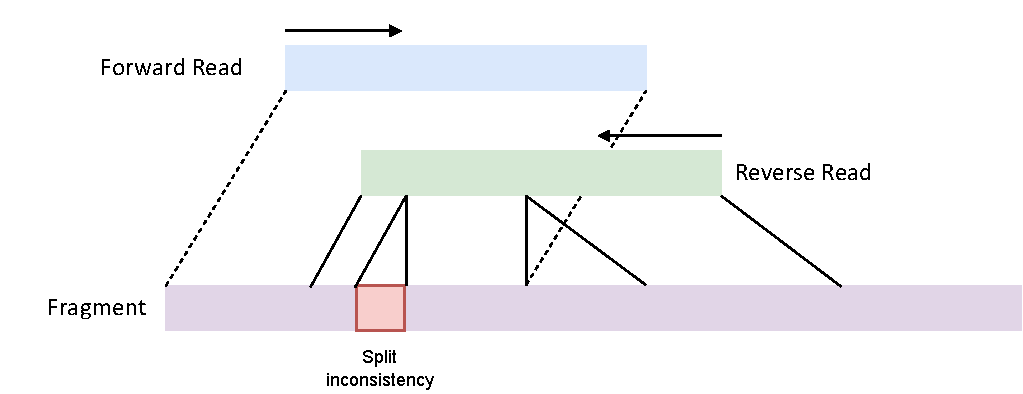
\includegraphics[width=0.5\textwidth]{figures/BamFeatures/overlapping-inconsistent-blocks}
        \caption
        {Diagram showing an example of an inconsistent read where the reads in a pair overlap but imply different introns (marked in red).}
        \label{fig:overlapping-inconsistent-blocks}
    \end{figure}

    \subsection{Read Mapping Types}
    A consistent read pair can either be \texttt{genic}, \texttt{intergenic}, or \texttt{intergenic containing}. A genic read pair is one where both reads in a par are contained within a gene. Formally speaking, that means all mapped bases of the read are $\geq$ gene start and $\leq$ gene end (with end-inclusive). A read pair is \texttt{intergenic} if it is not \texttt{genic}, and the read pair does not completely contain one or more genes. Containing a gene is defined as follows: the first mapped base of a read $\leq$ start of a gene and the last mapped base of a read $\geq$ end of the gene. All other read pairs are \texttt{intergenic-contained}.
    A \texttt{genic} read pair can either be \texttt{transcriptomic}, \texttt{merged-transcriptomic}, or \texttt{intronic}. A read pair is considered \texttt{transcriptomic} if it is fully contained within at least one annotated transcript and matches contiguously to a specific transcript section (Figure \ref{fig:transcriptomic-read}). This means that the intron boundaries observed in the read pair are consistent with those defined in the transcript annotation. Formally, a read pair matches a transcript if both read Region Vectors (RVs) are sub-RVs (defined later) of at least one transcript. A read pair is classified as \texttt{merged-transcriptomic} if it aligns to the merged transcript of a gene but does not necessarily match contiguously (Figure \ref{fig:merged-transcriptomic-read}). The merged transcript represents the union of all exonic regions of a gene, disregarding specific intron boundaries. This classification accounts for reads that may span novel isoforms or unannotated transcripts. Formally, a read pair matches the merged transcript if each base of the read pair aligns with some exon in the merged transcript. This broader definition enables the identification of potential new transcript variants while maintaining consistency with the gene’s exon structure. A read pair is classified as \texttt{intronic} if it is fully contained within the gene body but does not align to any annotated transcript or merged transcript (Figure \ref{fig:intronic-read}). Intronic reads may represent unprocessed RNA, novel isoforms with unannotated intron retention, or other transcriptional events within the gene body.

    Since we are only looking for the most biologically plausible explanation, we only want to consider the most plausible case (\texttt{transcriptomic} $>$ \texttt{merged-transcriptomic} $>$\texttt{intronic}). For example, if a read pair matches a specific transcript of one gene but also the merged transcript of another gene, we would only consider the transcriptomic match as it is more plausible. If a read pair matches multiple transcripts of multiple genes, we would want to know all the matched transcripts.
    \begin{figure}
        \centering
        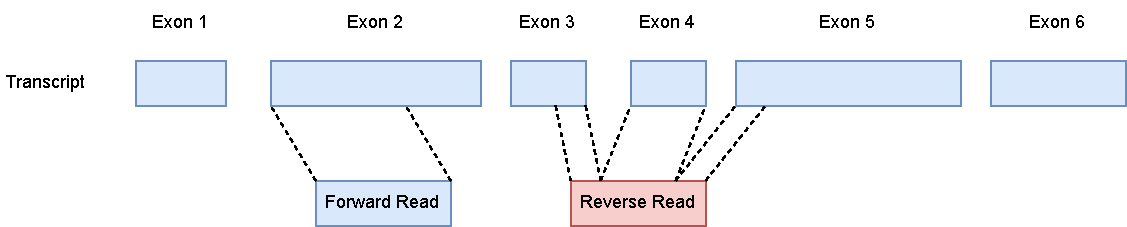
\includegraphics[width=0.7\textwidth]{figures/BamFeatures/transcriptomic-read}
        \caption
        {Diagram showing an example of a transcriptomic read pair. The read pair is fully contained within a gene and matches contiguously to a specific transcript section. The color indicates the strand}
        \label{fig:transcriptomic-read}
    \end{figure}
    \begin{figure}
        \centering
        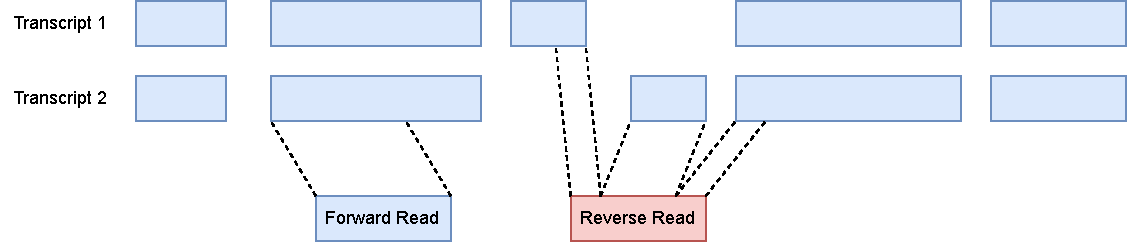
\includegraphics[width=0.7\textwidth]{figures/BamFeatures/merged-transcriptomic-read}
        \caption
        {Diagram showing an example of a merged transcriptomic read pair. The read pair aligns to the merged transcript of a gene but does not necessarily match contiguously. The color indicates the strand}
        \label{fig:merged-transcriptomic-read}
    \end{figure}
    \begin{figure}
        \centering
        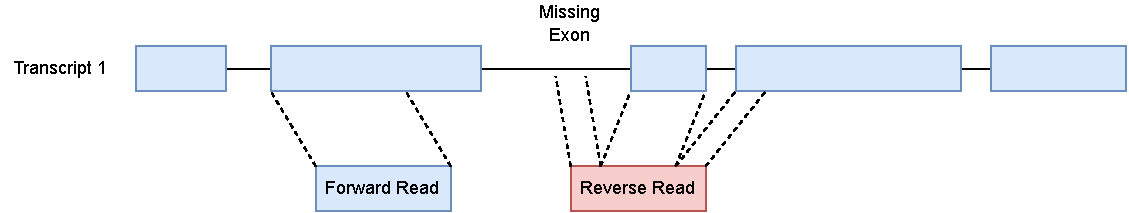
\includegraphics[width=0.7\textwidth]{figures/BamFeatures/intronic-read}
        \caption
        {Diagram showing an example of an intronic read pair. The read pair is fully contained within the gene body but does not align with any annotated transcript or merged transcript. The color indicates the strand.}
        \label{fig:intronic-read}
    \end{figure}

    \subsection{PCR Amplification}
    PCR amplification is a key step in RNA-seq library preparation, where DNA fragments are exponentially amplified to generate sufficient material for sequencing. While essential, this process can introduce biases, as some fragments are amplified more than others. A possible reason for this is because the process is exponential, if a fragment is amplified, it increases the chance that it will be amplified again. This continues exponentially and can lead to the overrepresentation of certain fragments, distorting the quantitative nature of RNA-seq data. The PCR index (\texttt{pcrindex}) is a metric used to identify read pairs that may have been amplified multiple times due to PCR cycles. It is calculated by tracking all observed read pairs and their associated regions (e.g., Region Vectors or \texttt{RV}s). If a read pair’s Region Vector matches previously observed regions, it is flagged as a potential PCR duplicate. This approach ensures that repeated fragments, whether arising from overamplification or technical artifacts, are systematically identified.
    There are multiple methods that are frequently used to address this distortion. Downsampling simply involves downweighting overamplified fragments. Barcoding fragments before PCR allows us to distinguish true biological duplicates from ones created due to PCR amplification. In this project, we will compare the results of all reads and those that are unique.

    \subsection{Test Files}
    To optimize computation time, the submission server will only verify the correctness of the program using small test
    files. Therefore, three large complete BAM files are provided for evaluation. The objective of the project is to
    process the \texttt{ebna\_hisat.bam}
    file within one hour while using a maximum of 10GB of RAM. Additionally, the read annotations of the test files will
    be analyzed. The other files used in this assignment are shown in Tables \ref{tab:test-bam-runtime} \&
    \ref{tab:reference-bam-runtime}.

    \subsection{Gene Expression Units}
    Gene expression levels in RNA sequencing are often quantified using standardized units that account for sequencing depth and gene length. One commonly used metric is Reads Per Kilobase of transcript per Million mapped reads (RPKM), which normalizes read counts to enable comparisons across genes and samples (Equation \ref{eq:rpkm})\cite{bedre_2021}. This metric is calculated per gene.
    \begin{figure}[h]
        \centering
        \begin{equation}
            RPKM = \frac{r \times 10^3 \times 10^6}{t \times l}
            \label{eq:rpkm}
        \end{equation}
        \caption{RPKM Formula with $r$ being the number of reads mapped to the gene, $t$ being the total number of mapped reads in the experiment, and $l$ being the length of the gene in base pairs (merged transcriptomic length). The factors $10^3$ and $10^6$ are used for scaling: $10^3$ to convert the length into kilobases (kb) and $10^6$ to normalize the read count per million mapped reads.}
    \end{figure}


    \section{Program Structure}

    \subsection{Program Usage}
    \begin{verbatim}
usage: java -jar bamfeatures.jar [-h] -gtf <gtf_file> -bam <bamfile>
                         -o <output_tsv> [-frstrand <true/false>]

named arguments:
  -h, --help             show this help message and exit
  -gtf <gtf_file>        GTF file
  -bam <bamfile>         BAM file
  -o <output_tsv>        Output file
  -frstrand <true/false>
                         true/false
    \end{verbatim}

    \subsection{Program Procedure}
    \begin{figure}[!htpb]
        \centering
        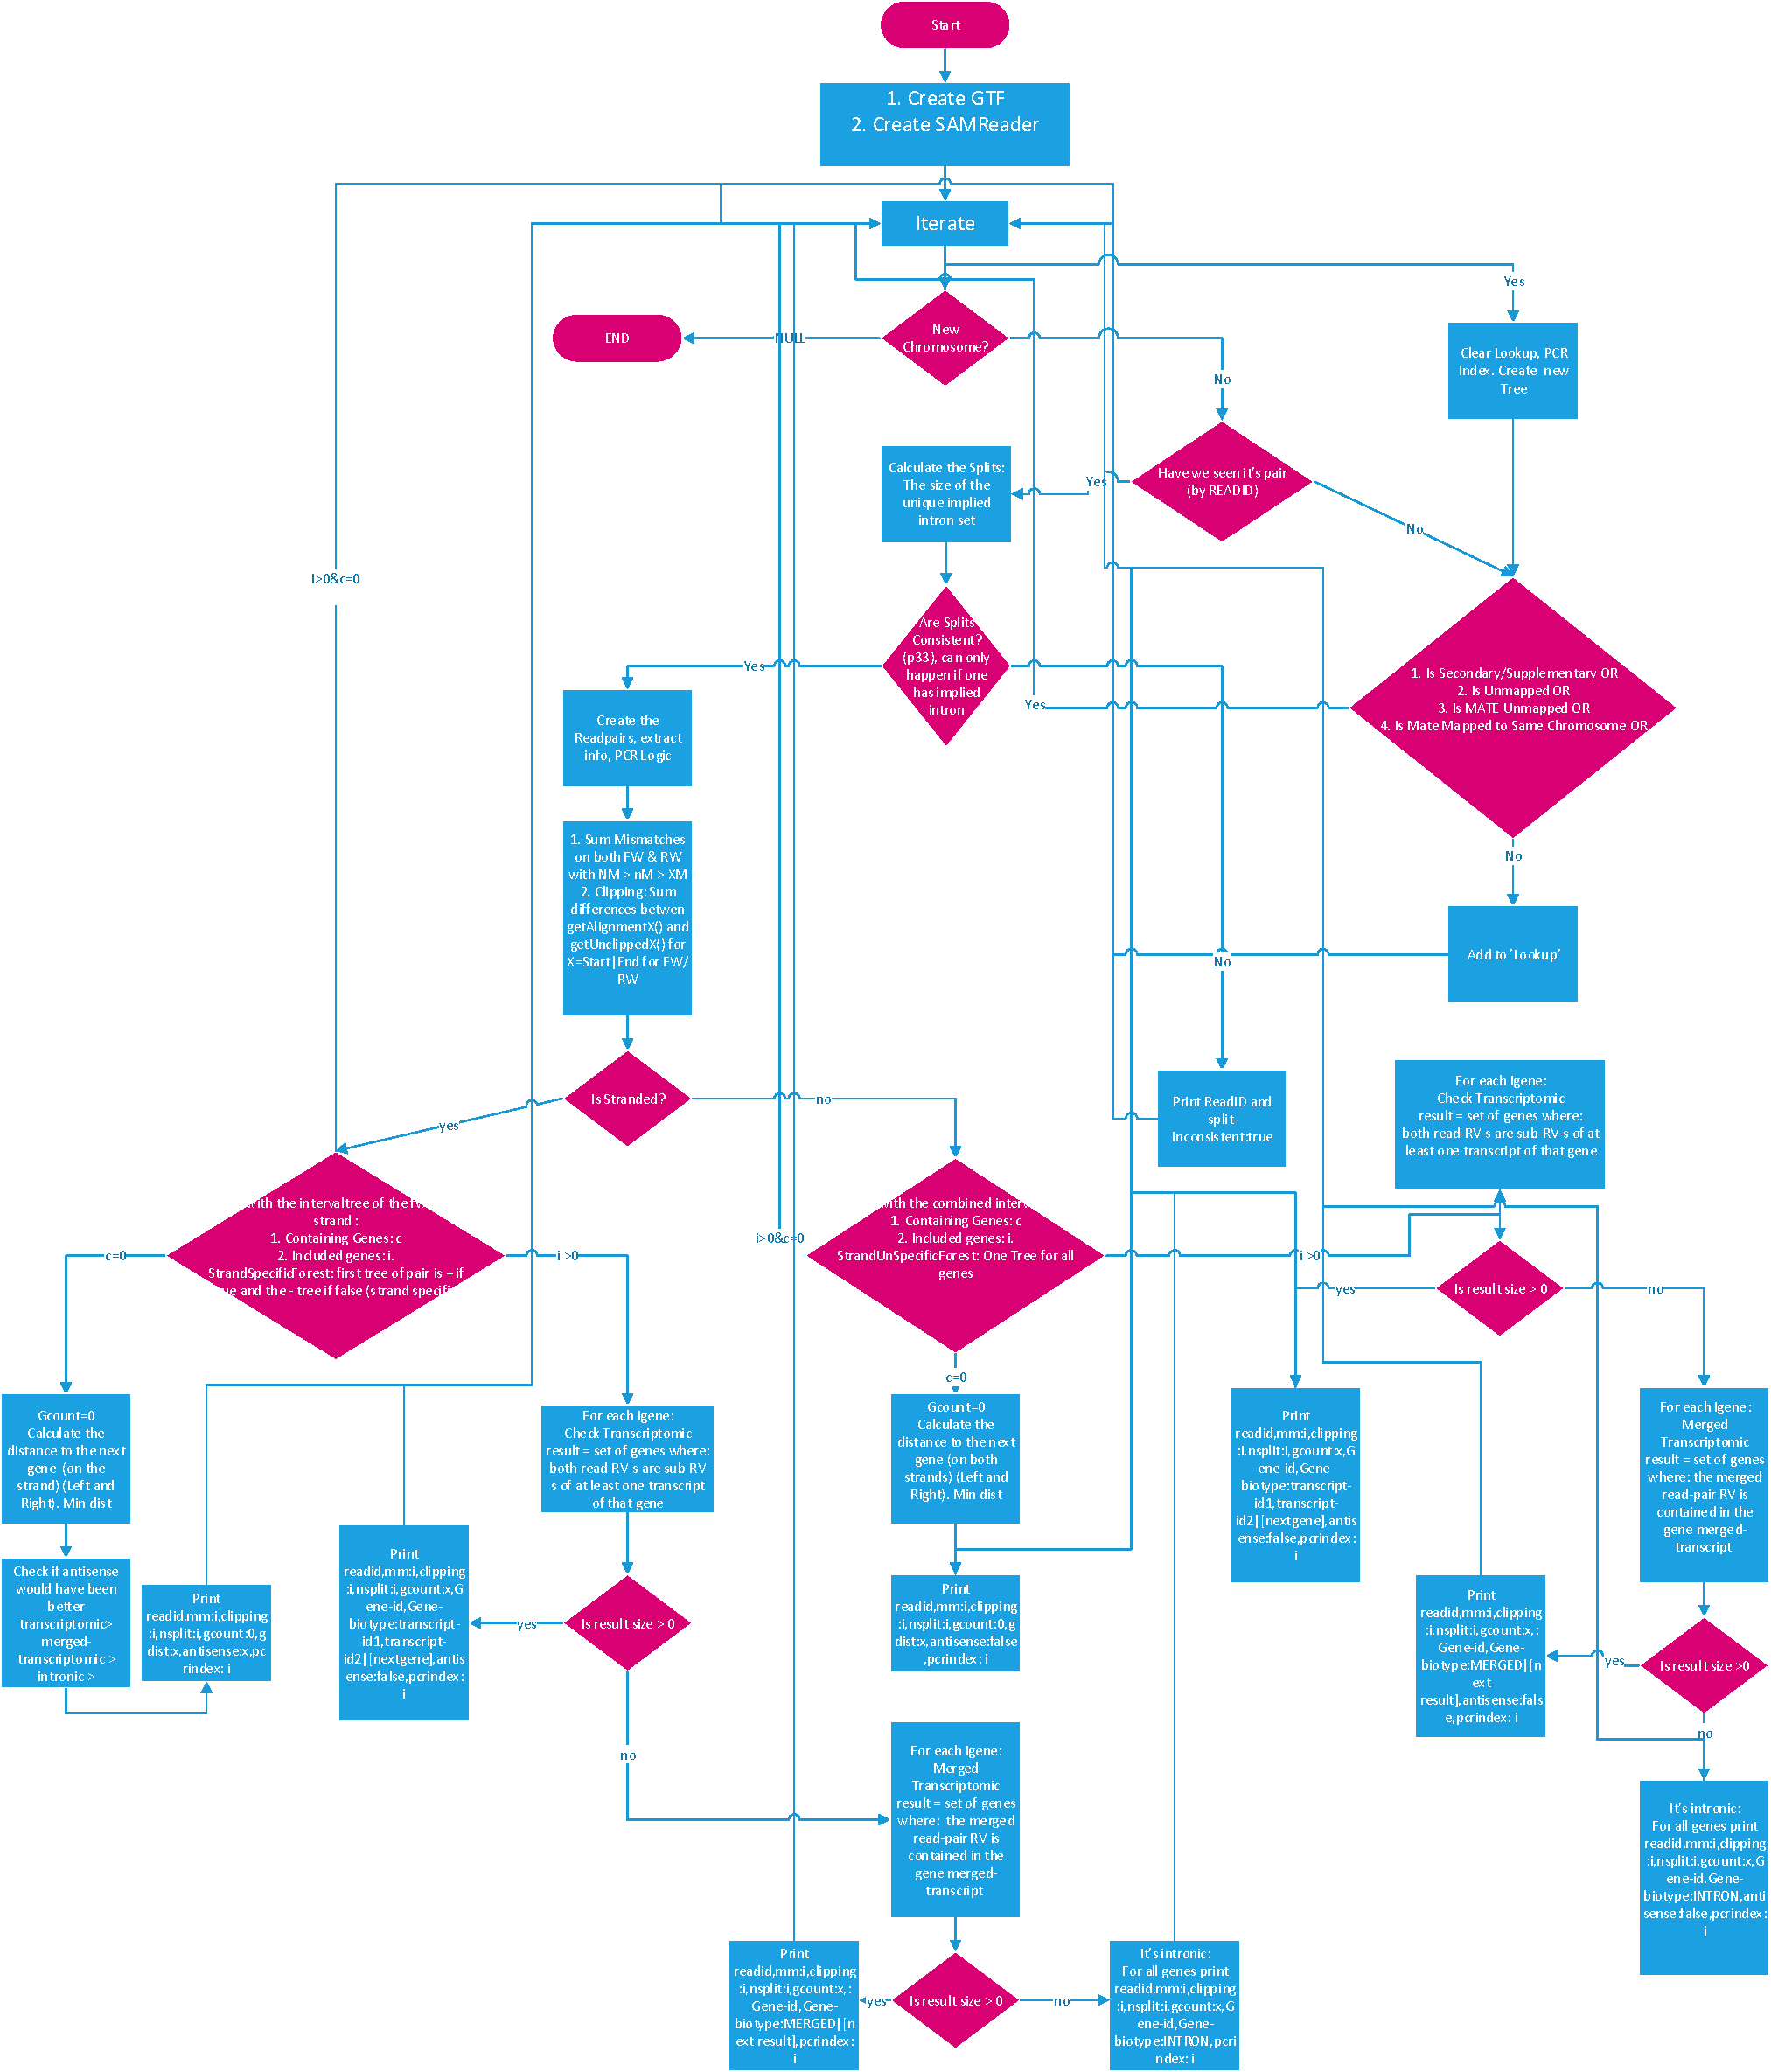
\includegraphics[width=0.7\textwidth]{figures/BamFeatures/BamFeaturesProcess-crop}
        \caption
        {Flowchart illustrating the logical program flow for solving the BamFeatures Assignment. Rectangles represent
        procedures, diamonds represent decisions,
            and rounded blocks represent start and endpoints. The process involves iterating through the BAM file and
            performing various checks and calculations. Once both forward and reverse reads have been found,
            the processing is performed.}
        \label{fig:program-procedure}
    \end{figure}
    Figure \ref{fig:program-procedure}
    shows the general process for solving the BamFeatures assignment. Due to the complexity of this assignment and the
    numerous cases, a flowchart is optimal for understanding the task. This allows optimal
    structuring of an implementation, as one can see which checks can be performed first, in order to possibly rule out
    other checks from needing to be made, saving computation time. The flowchart shows the process of processing a single read but differs from the actual implementation due to structural reasons. This is because the implementations processes the reads in batches (by chromosome), instead of one by one.

    \begin{enumerate}
        \item \textbf{Initialization and Setup}: Creation of the \texttt{ReadAnnotator} object, which initializes the \texttt{SamReader}, \texttt{IntervalTreeForestManager}, \texttt{PCRIndexManager} and various data structures to keep track of the reads to annotate.
        \item \textbf{Iteration Process}:
        \begin{enumerate}
            \item \textbf{Iterate through the SamReader}: Iterate to the next record, unless the end of the file is reached in which case go to step \ref{sec:last-chromosome-processing} \label{sec:iterate-samreader}
            \item \textbf{Chromosome Check}: Check if the current record is on the same chromosome as the previous record. If not, process the reads in step \ref{sec:new-chromosome-processing}. \label{sec:chromosome-check}
            \item \textbf{Valid Read Check}: Check conditions if the read is valid. If not, continue to step \ref{sec:iterate-samreader}.
            \item \textbf{Read Pair Check}: Check if we have seen the record's mate before:
            \begin{enumerate}
                \item If yes, add the records in the correct order (first of pair) to the readsToAnnotate List
                \item If no, add the record to the lookup table and continue to the next record.
            \end{enumerate}
            \item Go to step \ref{sec:iterate-samreader}.
        \end{enumerate}
        \item \textbf{New Chromosome Processing} \label{sec:new-chromosome-processing}:
        \begin{enumerate}
            \item \textbf{Read Processing}: \label{sec:read-processing}
            \begin{enumerate}
                \item Start two threads: Producer and Consumer.
                \item Producer iterates through the reads: \label{sec:producer}
                \item Check the \texttt{cgenes} and if empty then \texttt{igenes} for the read pair.
                \item If the read pair is genic ($\texttt{cgenes}>0$), check if it is \texttt{transcriptomic}, \texttt{merged-transcriptomic}, or \texttt{intronic}.
                \item If the read pair is intergenic ($\texttt{cgenes}=0 \land \texttt{igenes}=0$), get the distance to the next gene and check if the read pair is antisense matching
                \item Send the read pair to the consumer thread and go to step \ref{sec:producer}.
            \end{enumerate}
            \item Reset the data structures and return to step \ref{sec:chromosome-check}.
        \end{enumerate}
        \item \textbf{Last Chromosome Processing} \label{sec:last-chromosome-processing}:
        \begin{enumerate}
            \item Process the reads like in Step \ref{sec:read-processing}. Close the writer.
        \end{enumerate}
    \end{enumerate}
    During initialization, all the required data structures for processing are set up. Depending on whether the experiment is stranded or unstranded, the interval tree searching and PCR index processing are slightly different. However, these differences are only in the implementation, not in the core functionality. This provides an excellent opportunity to use an interface. Two interfaces are used: \texttt{IntervalTreeForestManager} and \texttt{PCRIndexManager}. Each has two implementations—one for strand-specific experiments and one for unstranded experiments.


    In a strand-specific experiment, two trees are used for each chromosome: one for each strand. This ensures that only the relevant strand is searched for a given read. In contrast, for an unstranded experiment, only one tree is needed, as both strands are always searched for the best match. As a result, the methods calculating \texttt{igenes}, \texttt{cgenes}, and \texttt{gdist} are all slightly different, but they essentially perform the same search. The \texttt{isAntisenseBetter} method always returns \texttt{false} in unstranded experiments, since both strands are already checked, whereas in stranded experiments, it performs an actual check. The \texttt{PCRIndexManager} also differs between stranded and unstranded experiments. In stranded experiments, it is important to ensure that the read maps to the exact location, including the strand. This requires maintaining two cache maps—one for each strand. The PCR index itself is organized as a \texttt{TreeSet} of region vectors, each corresponding to reads mapped to the PCR index. Crucially, the region vectors need to be "melted" (as explained later), because an alignment of (5,10) and (10,15) is considered equivalent to (5,15), and these should be counted together. When iterating through the \texttt{SAMRecords}, if the read is from a new chromosome, all reads from the previous chromosome are processed. Since the file is organized by chromosome and position, the PCR index and lookup data structures can be reset. The reads are processed using a producer-consumer pattern. Each record is then checked for validity. A read is considered valid only if all the following conditions are met:


    \begin{enumerate}
        \item The read is mapped
        \item The read is part of a pair
        \item The mate read is mapped
        \item The reads are on different strands
        \item The reads are on the same chromosome
        \item The read is not a supplementary alignment
    \end{enumerate}
    This check ensures that only valid reads are processed, guaranteeing the correctness of the annotation. Since both records of the first and second read in a pair are needed, processing cannot begin until both reads are found. A lookup table is used to match reads with their mates. If the mate has not been found yet, the read is added to the table using the read name, which is the same for paired reads but unique across the experiment. Once the mate is found, both reads are added to the \texttt{readsToAnnotate} list in the correct order. After processing the entire chromosome, all pairs in \texttt{readsToAnnotate} are annotated, and any remaining entries in the lookup table are ignored.


    The annotation of a read pair begins with extracting the alignment's start and end positions. These coordinates are then used to find the genes on the current chromosome and strand that fully include the read pair in their intervals. If any matching genes are found, the read pair is checked for genic properties. First, the alignment blocks of both reads are saved and "melted"—combining overlapping or neighboring blocks into a single block. For two region vectors, \(x\) and \(y\), if \(x_{\text{end}} \geq y_{\text{start}}\), a new region vector \(z\) is created as \(z \coloneqq (x_{\text{start}}, y_{\text{end}})\), for all combinations of \(x\) and \(y\). This ensures edge cases are handled correctly when calculating the PCR index, matching genes, and identifying splits. Afterward, consistency is checked by verifying that neither read contains a base from the implied intron of the other (see Figure X). This step also calculates the number of splits, which is saved directly. If the pair is consistent, basic read information such as clipping, mismatches, and PCR index is calculated.


    Next, the read is classified as transcriptomic, merged-transcriptomic, or intronic. To classify a read as transcriptomic, both reads' region vectors must be sub-region vectors of at least one transcript. A read region vector \(r\) is considered a sub-region vector of a transcript \(t\) if \(\text{cut}(t, r_{\text{start}}, r_{\text{end}}) = r\), as shown in Figure \ref{fig:transcriptomic-cut}. All matching transcripts are outputted, and the result of the cut operation is compared with the read vectors. If no match is found, a search for a merged transcript match is performed. A merged transcript is the union of all exonic regions of a gene. If both reads are contained within the merged transcript, the read is classified as a merged transcriptomic match. "Contained" means that every base of the read aligns to some exon in the merged transcript (see Figure \ref{fig:merged-transcriptomic-contained}). If no merged transcript match is found, the read is classified as intronic.


    If no gene or merged transcript contains the read, an intergenic check is performed. The interval tree is searched to see if the read pair fully contains a gene. If so, the read is ignored. The same checks as for the genic case are applied, but the gene distance is also calculated, and antisense matches are checked. Gene distance is determined by finding the nearest gene on the same strand, while antisense matches are checked by searching the interval tree for the antisense strand. If a genic match is found on the antisense strand, the read pair is classified as an antisense match. The PCR index is calculated by looking up the region vectors in the cache map. If the region vectors are found, the PCR index is outputted and iterated. Finally, the read pair is outputted.

    \begin{figure}[!htpb]
        \centering
        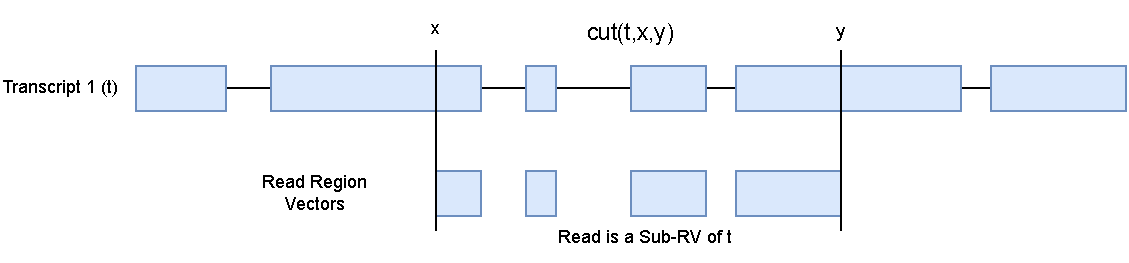
\includegraphics[width=0.7\textwidth]{figures/BamFeatures/transcriptomic-cut}
        \caption
        {Diagram showing how the cut method works for checking if a read matches a transcript. The transcript is cut starting from the first base of the read and ending at the last base of the read. If the cut transcript is the same as the read, the read matches the transcript.}
        \label{fig:transcriptomic-cut}
    \end{figure}

    \begin{figure}[!htpb]
        \centering
        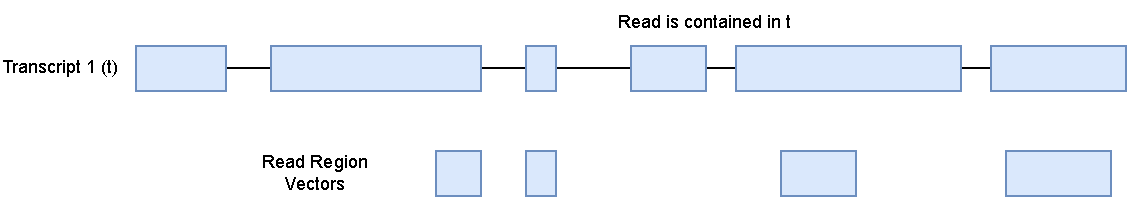
\includegraphics[width=0.7\textwidth]{figures/BamFeatures/merged-transcriptomic-contained}
        \caption
        {Diagram showing how contained works for checking if a read matches a merged transcript. The read is contained in the merged transcript if each base of the read aligns to some exon in the merged transcript.}
        \label{fig:merged-transcriptomic-contained}
    \end{figure}

    \subsection{Output Format}
% The output should contain one line per read pair in the format
% readid<tab>annotation.
% Rest of output depends on what feature the read has
    The output is structured in a TSV, with each line representing one read pair with the first column representing the read ID. The rest of the annotation is dependent on what type of annotation it is. Only valid reads that are \texttt{genic} or \texttt{intergenic} are outputted. If they are inconsistent we annotate with \texttt{split-inconsistent:true}. If not, we annotate the general statistics:
    \begin{itemize}
        \item \textbf{Mismatch count}: \texttt{mm:<mismatch-count>}
        \item \textbf{Clipping size}: \texttt{clipping:<clipping-count>}
        \item \textbf{Split count}: \texttt{nsplit:<split-count}
        \item \textbf{Gene count}: \texttt{gcount:<gene-count>}
    \end{itemize}
    If the read is genic, we also output the following depending on the match level:
    \begin{itemize}
        \item \textbf{Transcriptomic}: \texttt{<gene-id1>,<gene-biotype1>:<transcript-id1>,...|[gene-2...]}
        \item \textbf{Merged-Transcriptomic}: \texttt{<gene-id1>,<gene-biotype1>:MERGED|[gene-2...]}
        \item \textbf{Intronic}: \texttt{<gene-id1>,<gene-biotype1>:INTRON|[gene-2...]}
    \end{itemize}
    If it is intergenic, we output the gene distance (the distance to the next sense gene): \texttt{gdist:<gene-distance>} and whether the read pair matches a gene on the other strand \texttt{antisense:true|false} (If it is a strand unspecific experiment, it is always false).
    Additionally, we output the PCR index of the read pair (i.e.\ the number of read-pairs mapped exactly to the same genomic region as this read pair so far): \texttt{pcrindex:<pcrindex>}.


    \section{Analysis}
    The following analysis was performed with the sample files \texttt{ebna\_hisat.bam} and \texttt{hes\_star.bam} using \texttt{Homo\_sapiens.GRCh37.75.gtf}, and \texttt{nookaew\_cm.bam} using \texttt{Saccharomyces\_cerevisiae.R64-1-1.75.gtf}. The program was run using the specified strandness from the reference table on the Biocluster grid. The files were queued with \texttt{QueueGridForRefTable.sh} and analyzed with \texttt{QueueGridForAnalyze.sh} using \texttt{bamfeatures.jar} and \texttt{AnalyzeBAMFeatures.py} respectively.

    \subsection{Correctness}

    \subsubsection{RPKM Distribution}
    %
%over all detected genes both considering all reads or only non-PCR duplicated reads (PCR index
%= 0)

    The \texttt{RPKM} values were calculated for all genes mapped in the three provided analysis files using the formula in Figure \ref{eq:rpkm}. The \texttt{RPKM} values were calculated for all reads and for unique reads (non-PCR amplified reads) separately. The distribution of the \texttt{RPKM} values was then plotted on a log scale for each file. The distribution of the \texttt{RPKM} values for all reads, and unique reads are shown in Figure \ref{fig:rpkm-distribution}. The distribution of the \texttt{RPKM} values for the top 10 genes in each file is shown in Figure \ref{fig:rpkm-scatter}. The comparison of the \texttt{RPKM} values for all reads and unique reads is shown in Figure \ref{fig:total-vs-unique-scatter}. We can see that the unique \texttt{RPKM} values are lower than the total \texttt{RPKM} values with \texttt{hes\_star} and \texttt{ebna\_hist} having a larger difference than \texttt{nookaew\_cm}.
    % log rpkm distribution
    \begin{figure}[!htbp]
        \centering
        \begin{minipage}{0.48\textwidth}
            \centering
            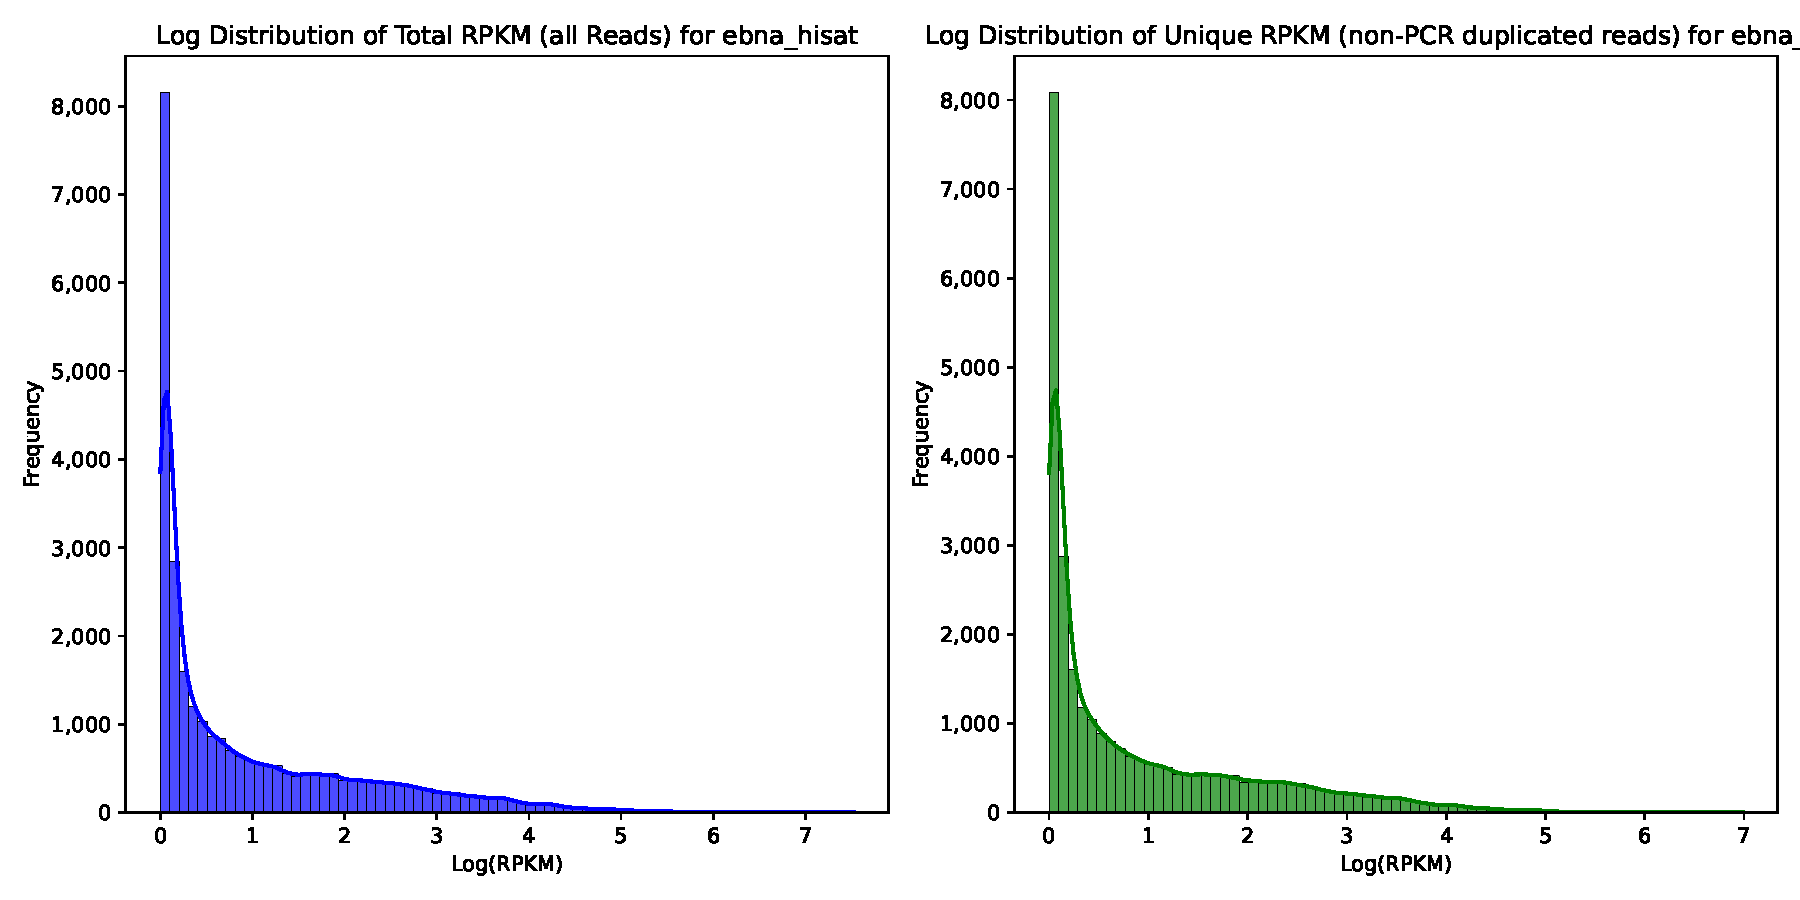
\includegraphics[width=\textwidth]{figures/BamFeatures/annot/ebna_hisat_log_rpkm_distribution}
            \label{fig:ebna_hisat_log_rpkm_distribution}
        \end{minipage}
        \hfill
        \begin{minipage}{0.48\textwidth}
            \centering
            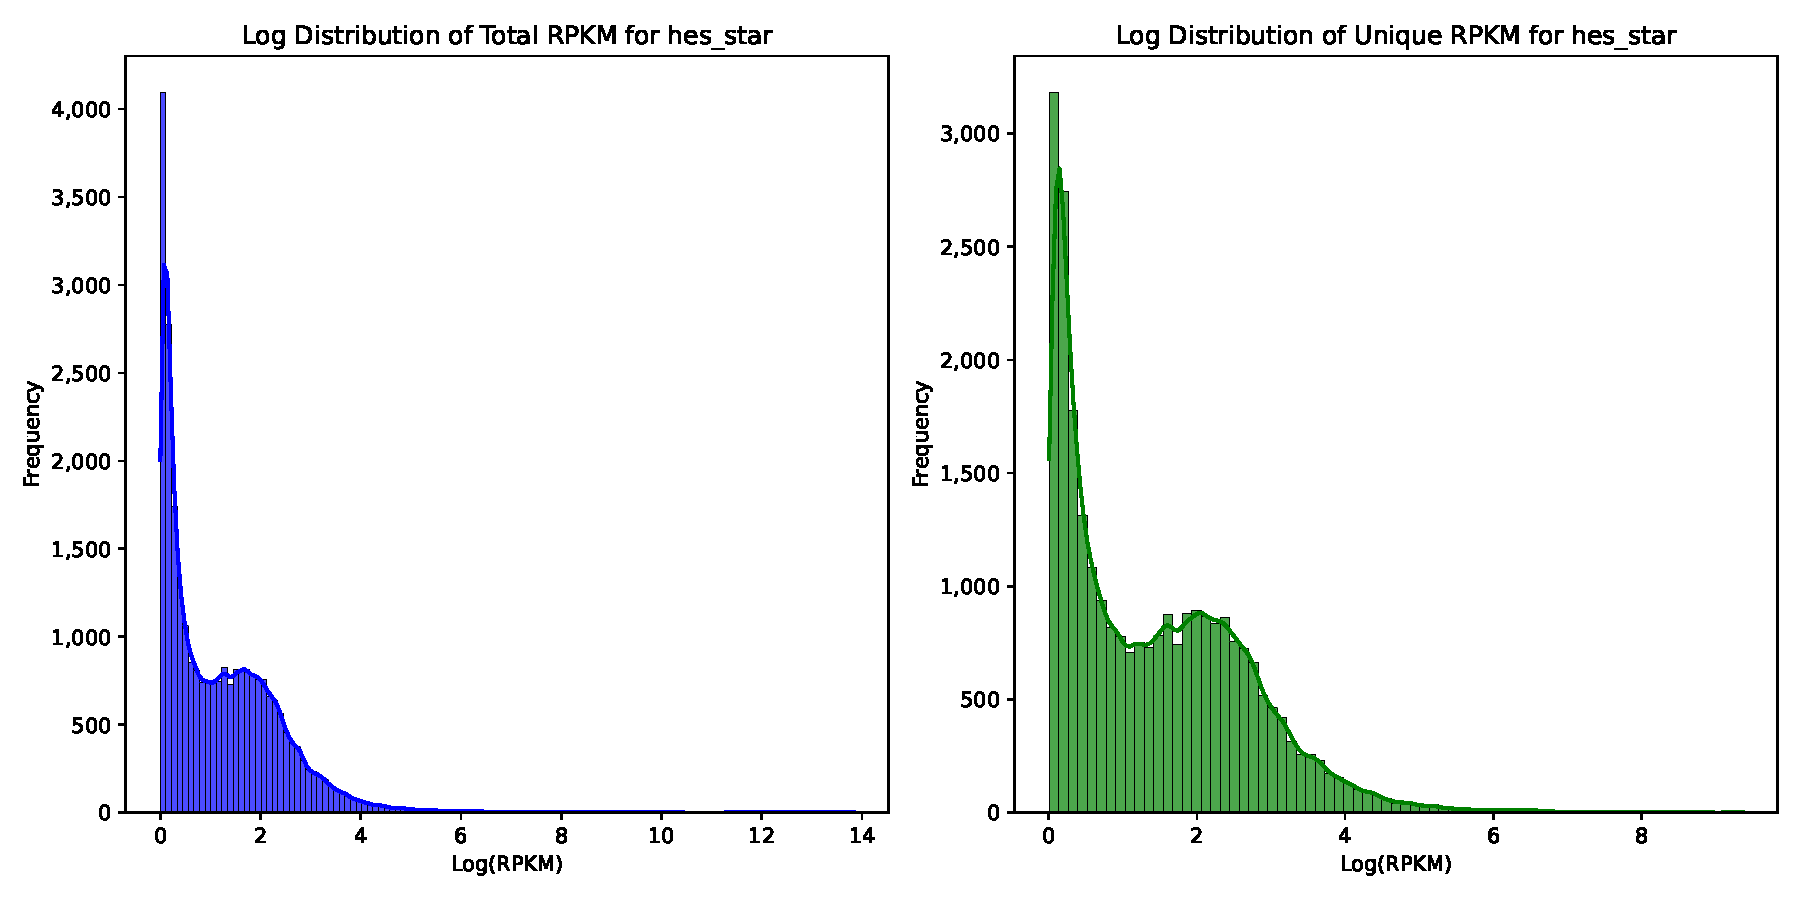
\includegraphics[width=\textwidth]{figures/BamFeatures/annot/hes_star_log_rpkm_distribution}
            \label{fig:hes_star_log_rpkm_distribution}
        \end{minipage}

        \begin{minipage}{0.48\textwidth}
            \centering
            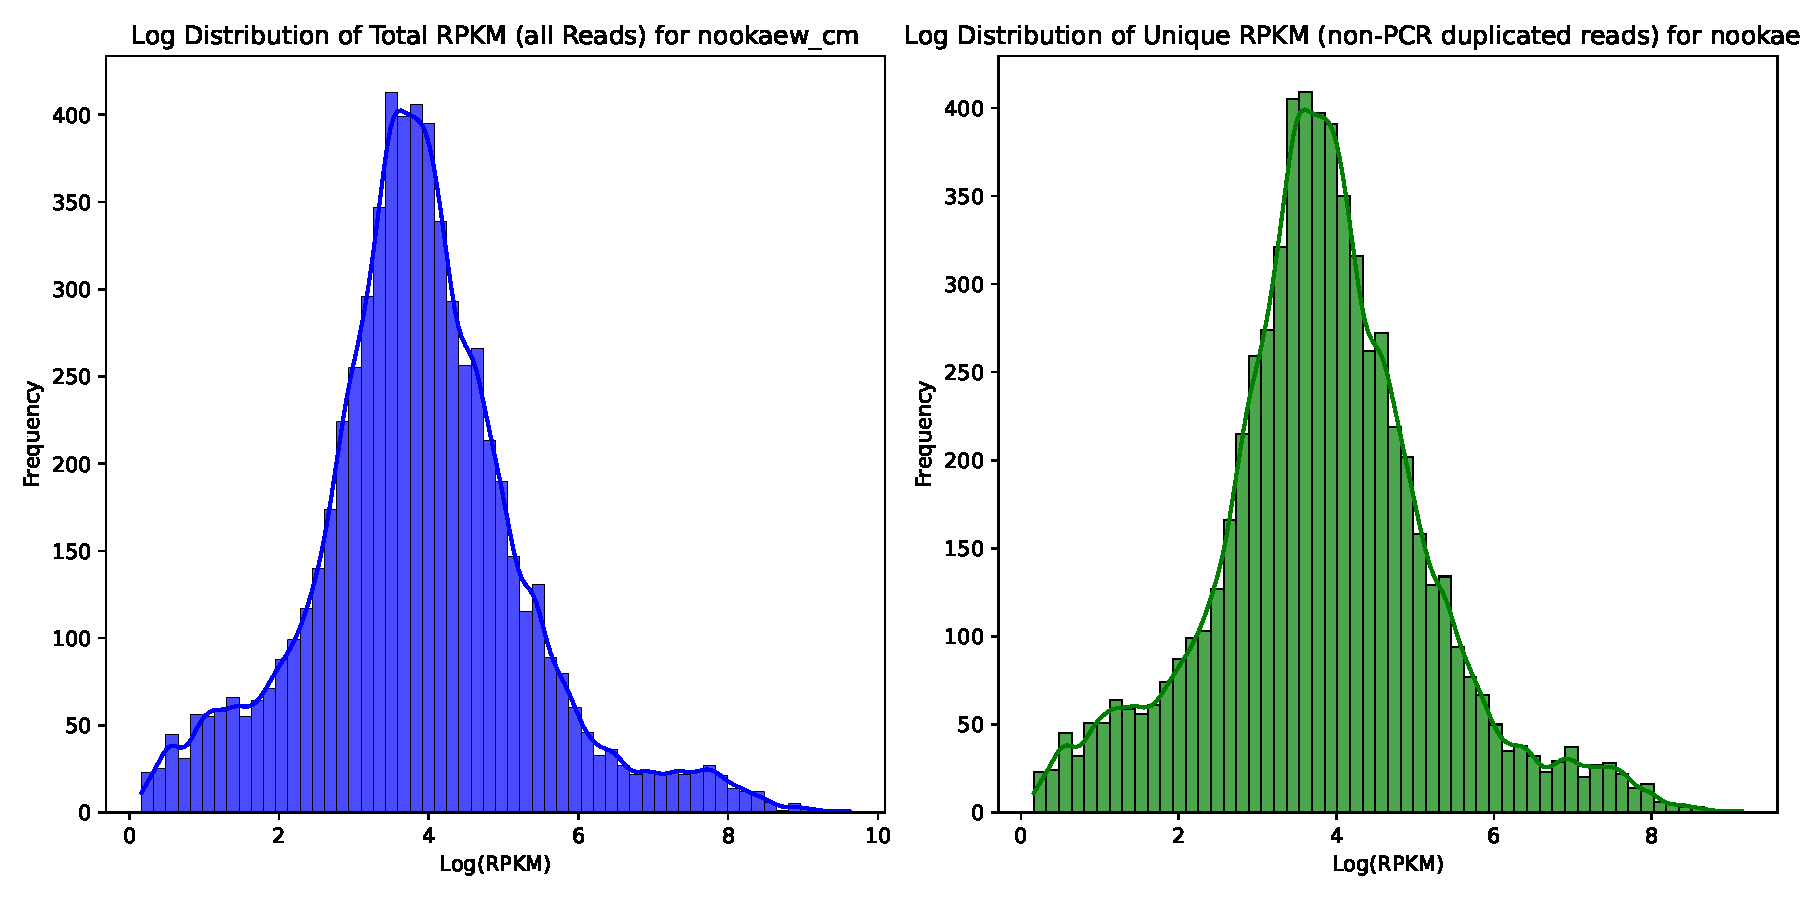
\includegraphics[width=\textwidth]{figures/BamFeatures/annot/nookaew_cm_log_rpkm_distribution}
            \label{fig:nookaew_cm_log_rpkm_distribution}
        \end{minipage}
        \caption{Log distribution of the total (all reads) vs unique (non-PCR amplified) RPKM values for the provided analysis files with the kernel density function overlayed. Bin size is determined by the minimum of the sturges and fd estimators. The RPKM values get smaller in the unique case.}
        \label{fig:rpkm-distribution}
    \end{figure}

    Figure \ref{fig:rpkm-distribution} presents the log-transformed distribution of \texttt{RPKM} values for all genes in each dataset, overlayed with a kernel density estimate (KDE). The bin size was chosen based on the minimum of the Sturges and Freedman-Diaconis estimators to achieve an optimal balance between resolution and interpretability. The unique (non-PCR amplified) \texttt{RPKM} values are lower than the total \texttt{RPKM} values, indicating the removal of duplicated reads likely due to PCR amplification. The magnitude of this difference varies across datasets, reflecting differences in sequencing quality, depth, and library preparation protocols. However, it demonstrates the importance of this correction step in ensuring accurate gene expression quantification while noting that the unique \texttt{RPKM} values are overcorrecting for true biological replicates (as explained earlier). For the following analysis, we will only consider the result genes for the unique \texttt{RPKM} values (Figure \ref{fig:rpkm-scatter}, green plot). The top gene for the \texttt{hes\_star} experiment, \href{https://grch37.ensembl.org/Homo_sapiens/Gene/Summary?g=ENSG00000210082;r=MT:1671-3229;t=ENST00000387347}{ENSG00000210082}, codes for the mitochondrial 16sRNA. The top few genes for \texttt{nookaew\_cm} are all related to Glycolosis like \href{https://www.yeastgenome.org/locus/S000003424}{YGR192C} which codes for Glyceraldehyde-3-phosphate dehydrogenase (GAPDH), \href{https://www.yeastgenome.org/locus/S000001543}{YKL060C} which codes for Fructose 1,6-bisphosphate aldolase, and \href{https://www.yeastgenome.org/locus/S000001217}{YHR174W} which codes for ENOlase. Similarly to \texttt{hes\_star}, the top genes for \texttt{ebna\_hist} are mostly noncoding RNAs, such as \href{https://grch37.ensembl.org/Homo_sapiens/Gene/Summary?db=core;g=ENSG00000249335;r=5:68128412-68257985;t=ENST00000503268}{ENSG00000249335} and \href{https://grch37.ensembl.org/Homo_sapiens/Gene/Summary?db=core;g=ENSG00000256725;r=12:131112861-131200826}{ENSG00000256725} which are LincRNAs.

    % TODO Names cut off the top of plot, better naming

    % TODO: better caption
    %rpkm scatter
    \begin{figure}[!htbp]
        \centering
        \begin{minipage}{0.48\textwidth}
            \centering
            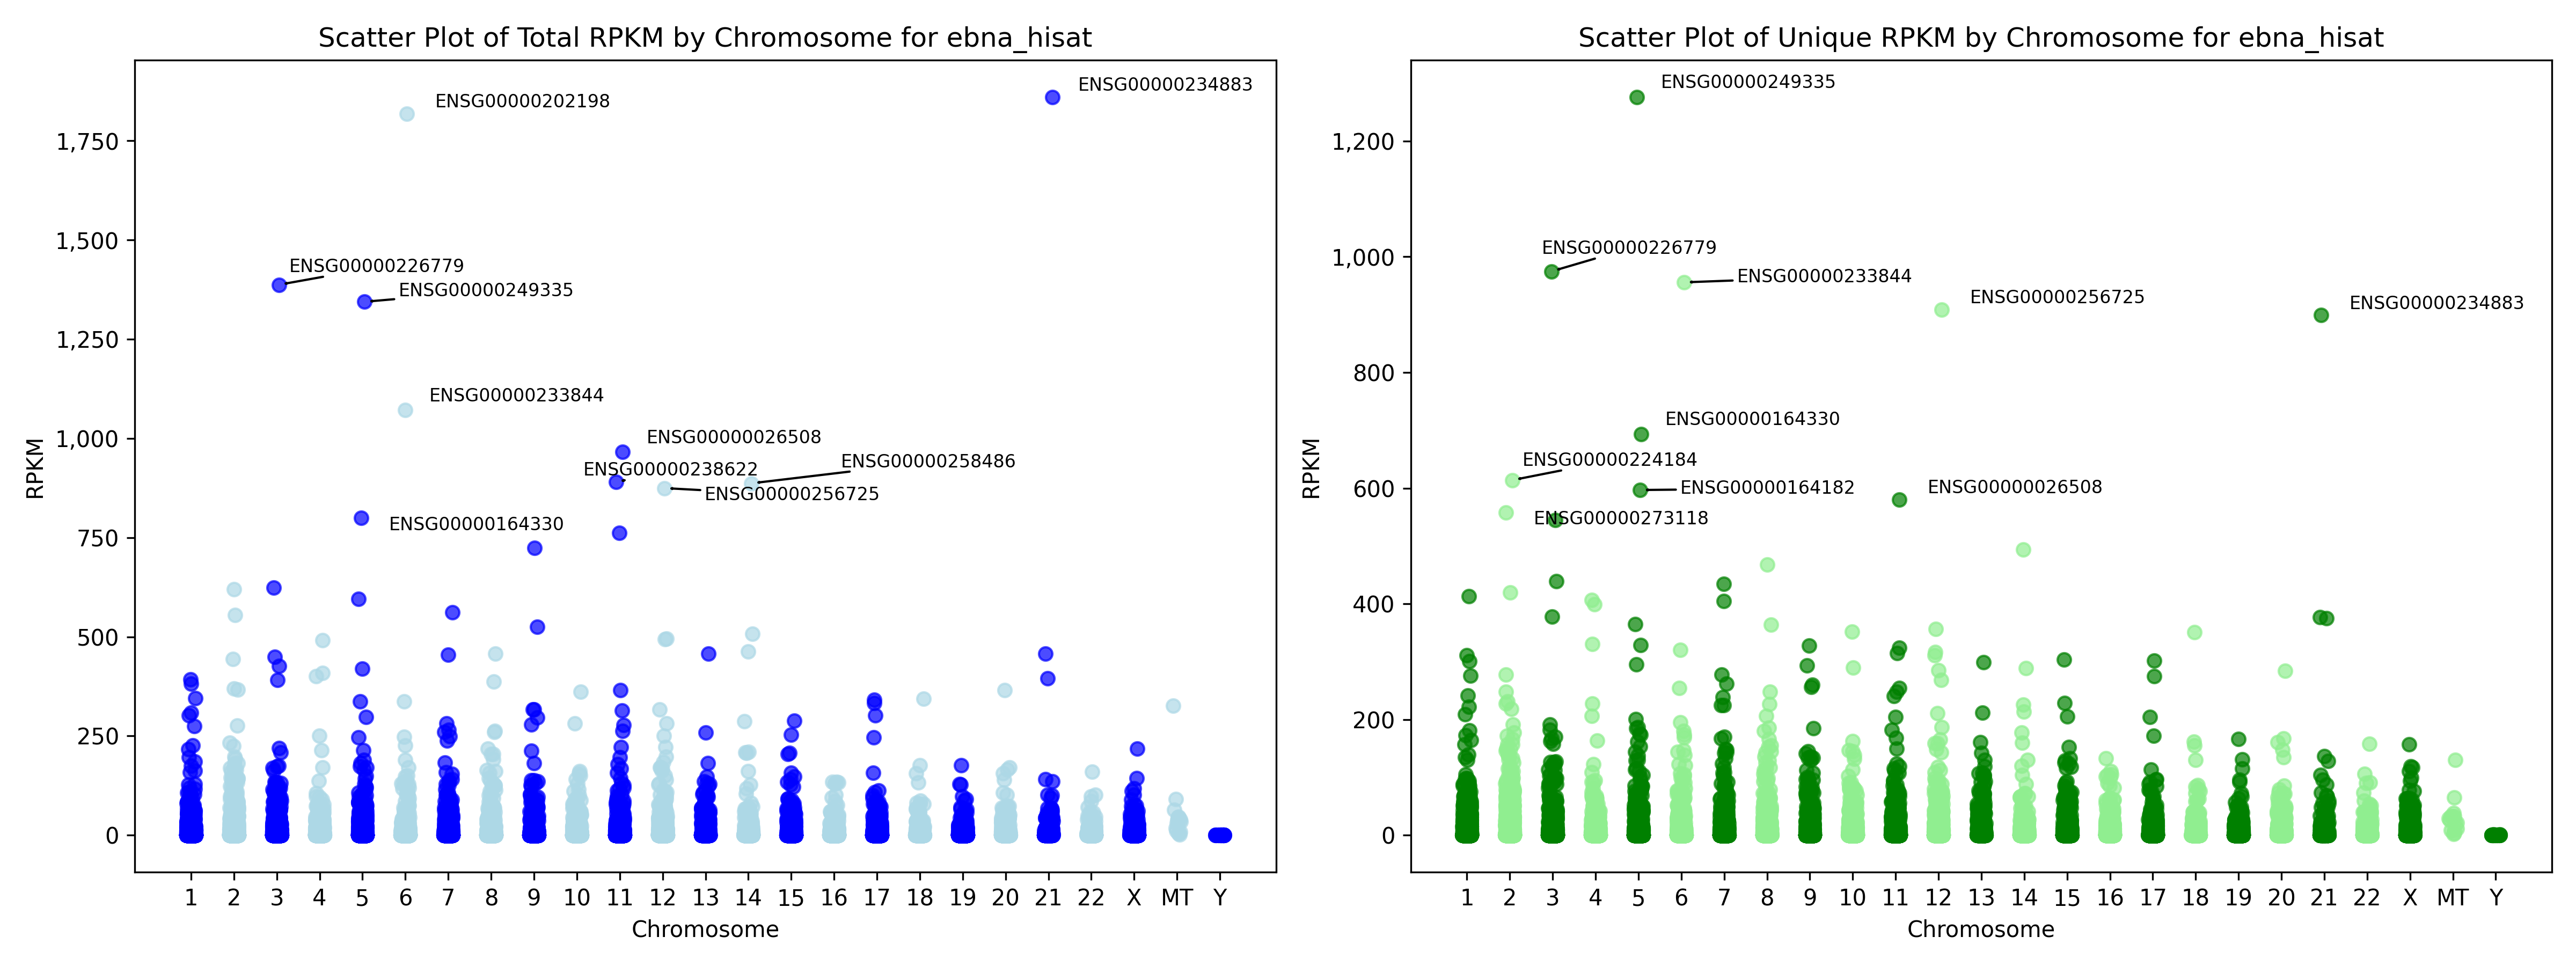
\includegraphics[width=\textwidth]{figures/BamFeatures/annot/ebna_hisat_rpkm_scatter}
            \label{fig:ebna_hisat_rpkm_scatter}
        \end{minipage}
        \hfill
        \begin{minipage}{0.48\textwidth}
            \centering
            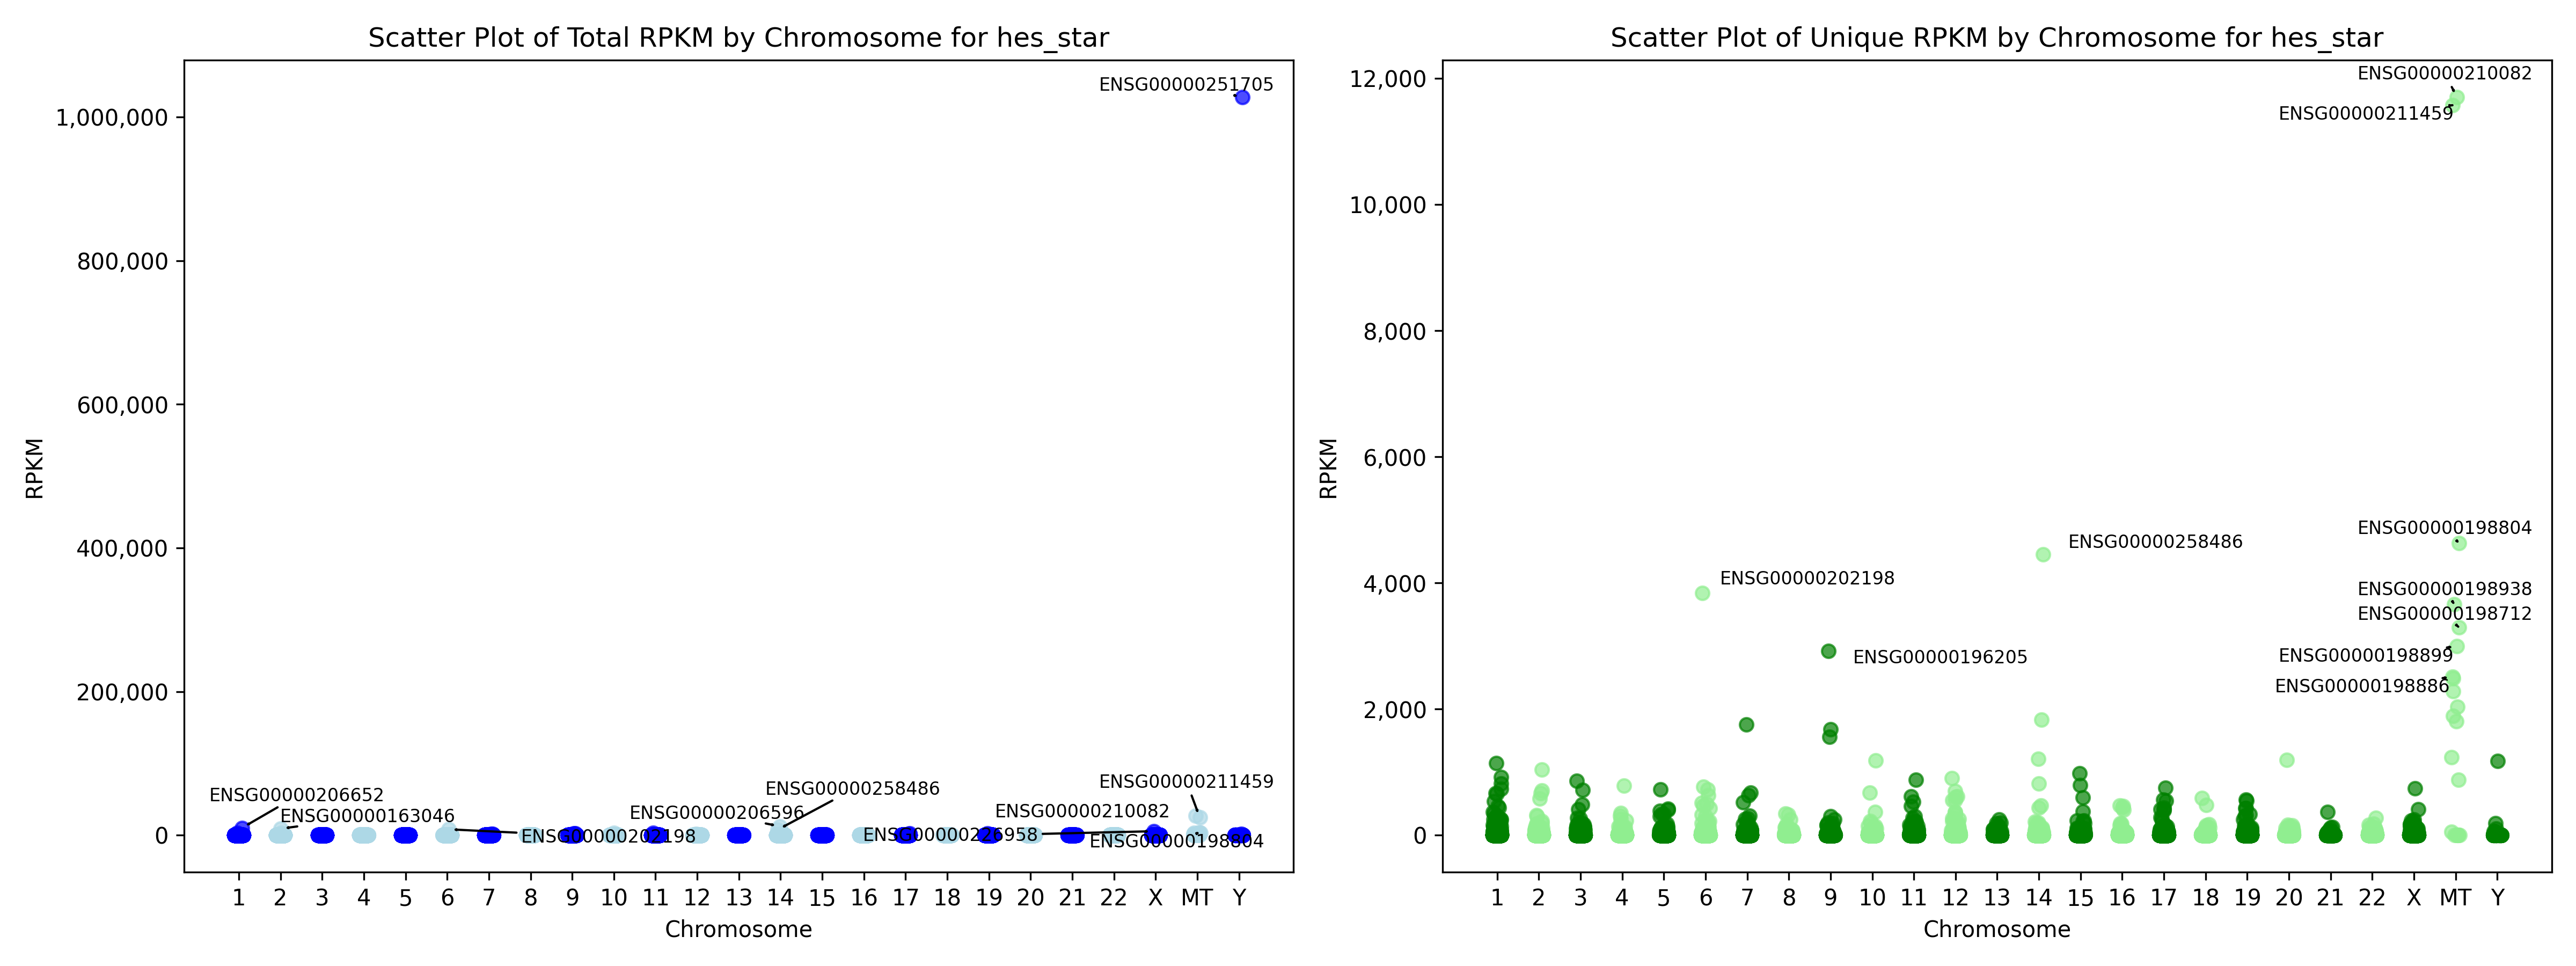
\includegraphics[width=\textwidth]{figures/BamFeatures/annot/hes_star_rpkm_scatter}
            \label{fig:hes_star_rpkm_scatter}
        \end{minipage}
        \begin{minipage}{0.48\textwidth}
            \centering
            \includegraphics[width=\textwidth]{figures/BamFeatures/annot/nookaew_cm_rpkm_scatter}
            \label{fig:nookaew_cm_rpkm_scatter}
        \end{minipage}
        \caption{Scatter plot of the total (all reads) vs unique (non-PCR amplified) RPKM values for the provided analysis files separated by chromosome. The top 10 genes are labeled. The unique transformation greatly changes \texttt{hes\_star}, as it has an extreme outlier RN5-8S6, a ribosomal pseudogene. \texttt{nookaew\_cm} is more consistent and barely changes the top 10, with most being gene coding for proteins in Glycolysis. \texttt{ebna\_hisat} has a few outliers, but the top 10 are mostly the same and also rRNAs.}
        \label{fig:rpkm-scatter}
    \end{figure}
    %rpkm unique vs total scatter
    \begin{figure}[!htbp]
        \centering
        \begin{minipage}{0.32\textwidth}
            \centering
            \includegraphics[width=\textwidth]{figures/BamFeatures/annot/ebna_hisat_log_total_rpkm_vs_unique_scatter}
            \label{fig:ebna_hisat_log_total_rpkm_vs_unique_scatter}
        \end{minipage}
        \hfill
        \begin{minipage}{0.32\textwidth}
            \centering
            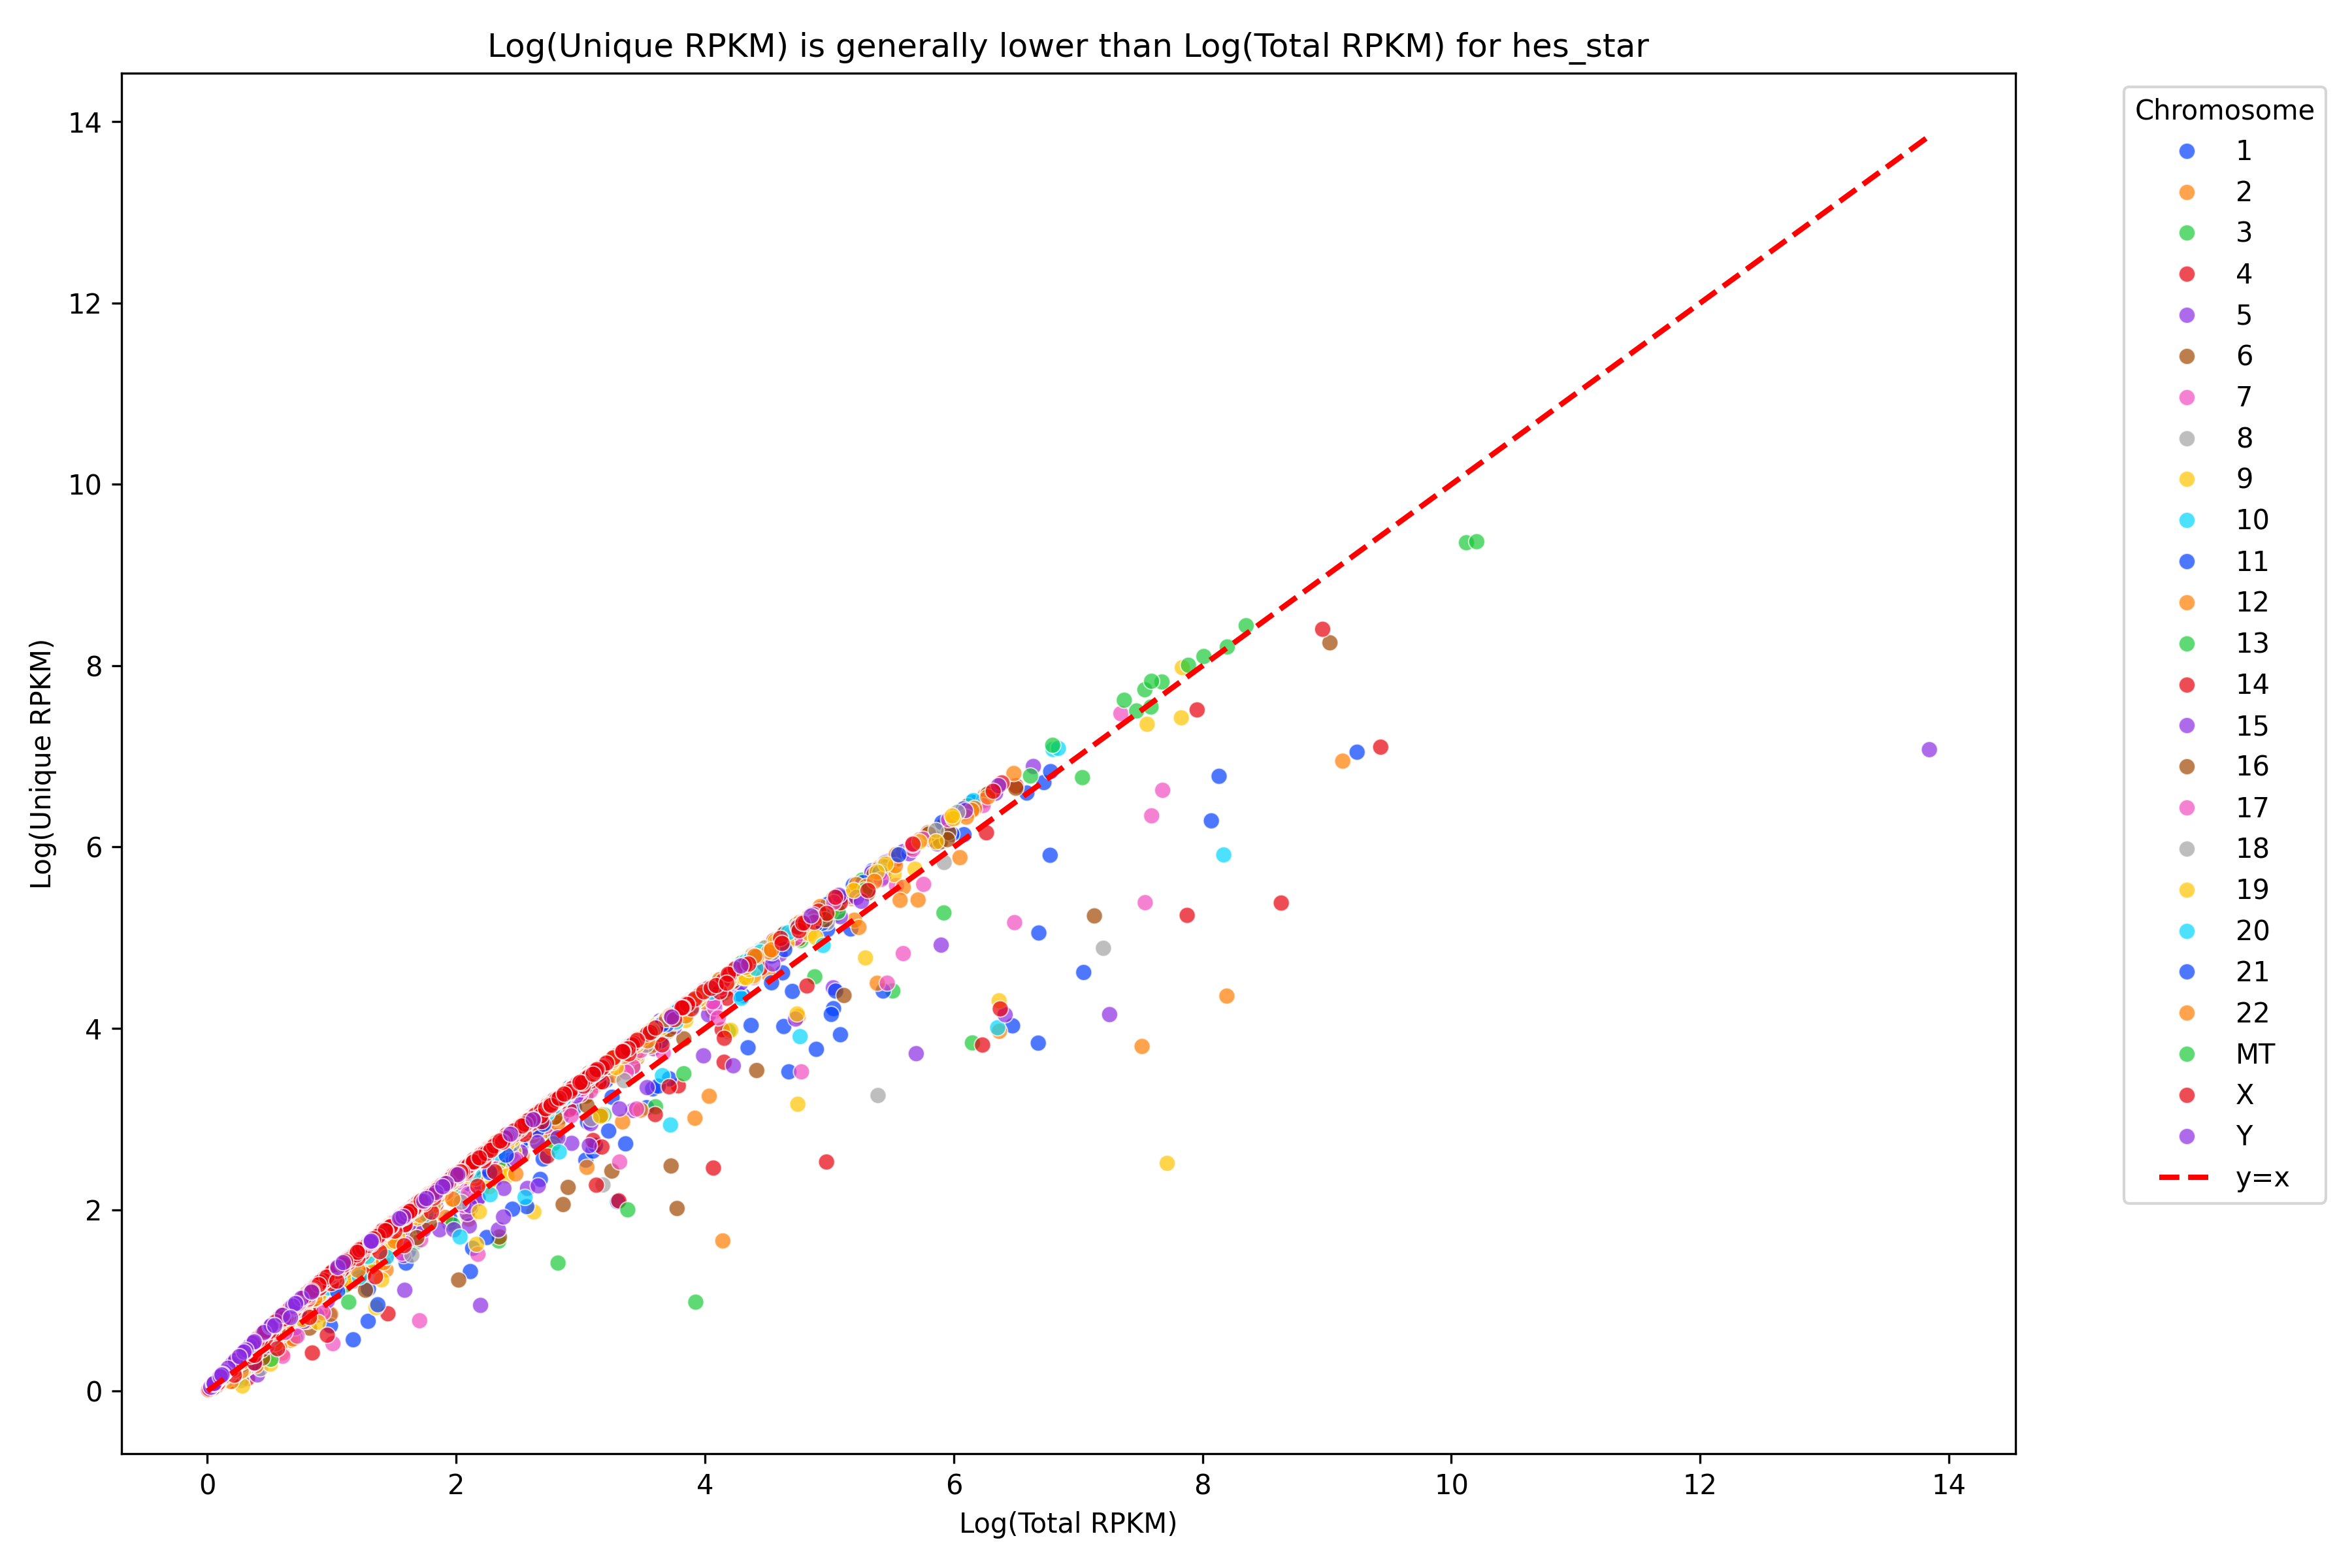
\includegraphics[width=\textwidth]{figures/BamFeatures/annot/hes_star_log_total_rpkm_vs_unique_scatter}
            \label{fig:hes_star_log_total_rpkm_vs_unique_scatter}
        \end{minipage}
        \hfill
        \begin{minipage}{0.32\textwidth}
            \centering
            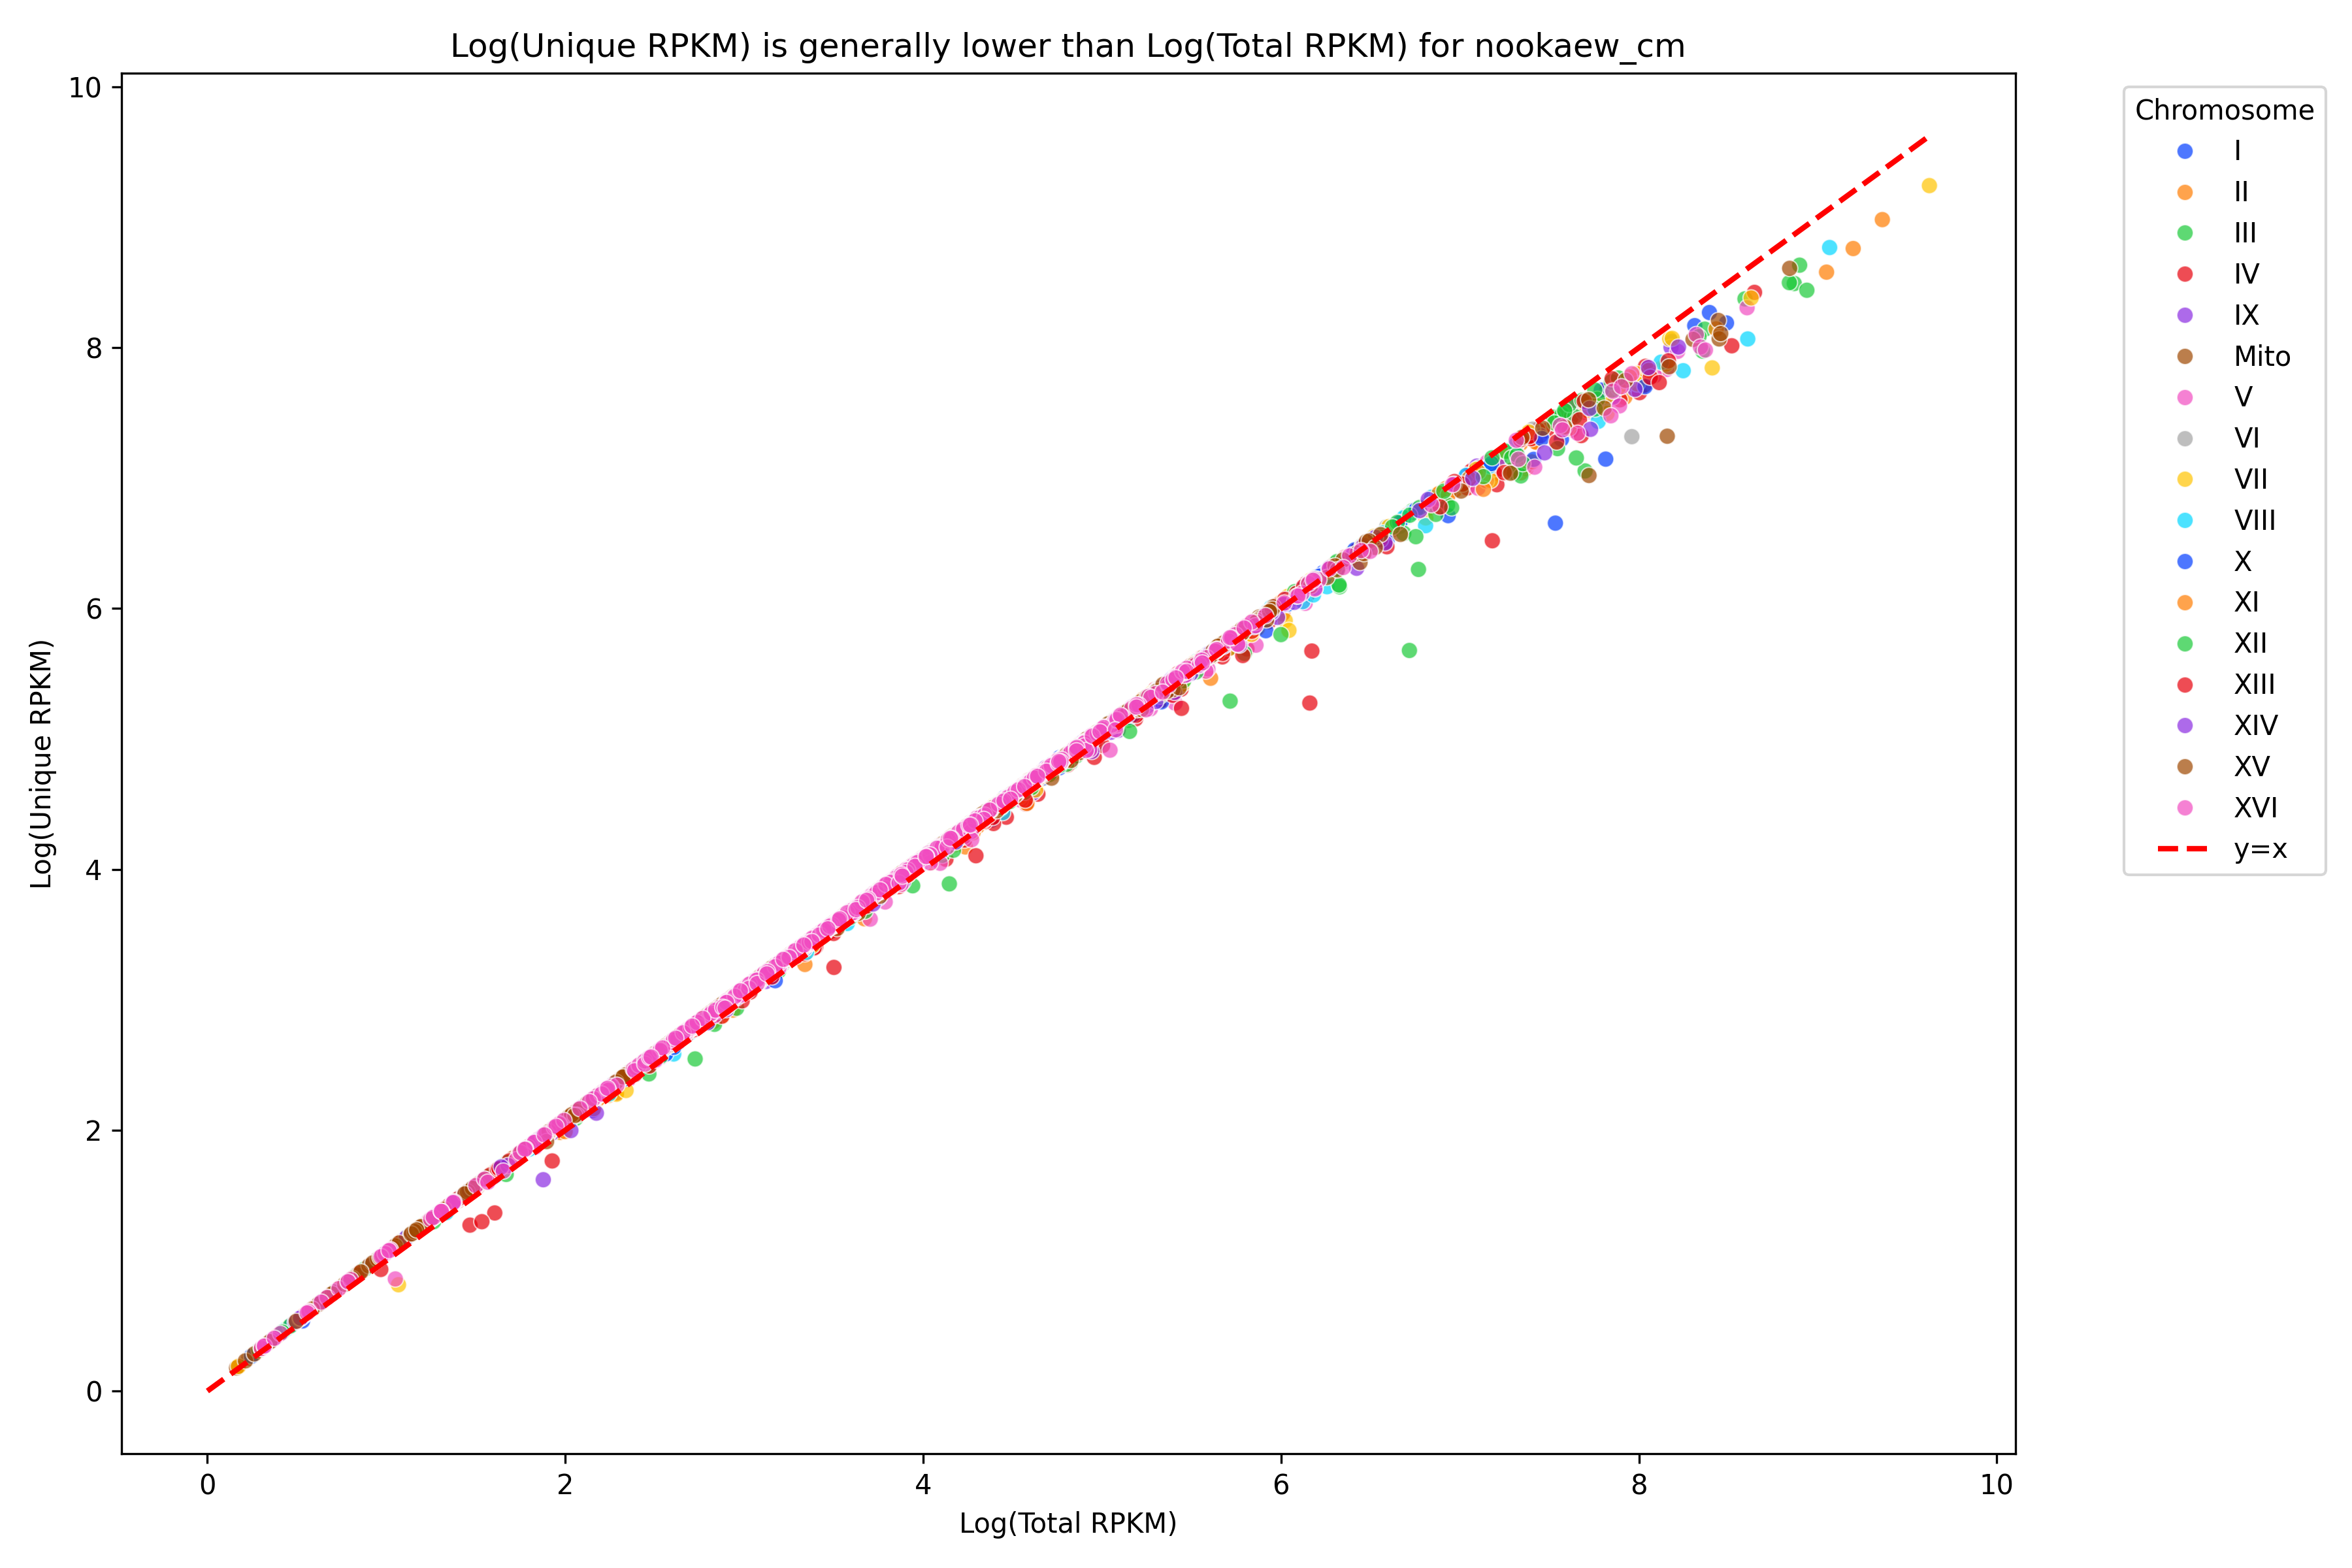
\includegraphics[width=\textwidth]{figures/BamFeatures/annot/nookaew_cm_log_total_rpkm_vs_unique_scatter}
            \label{fig:nookaew_cm_log_total_rpkm_vs_unique_scatter}
        \end{minipage}
        \caption{Comparison of log-transformed Unique RPKM and Total RPKM values for the provided analysis files. Each scatter plot represents genes grouped by their chromosomes, with the dashed red line indicating the $y=x$ diagonal, where Unique RPKM equals Total RPKM. Points below the diagonal indicate that Unique RPKM is lower than Total RPKM, reflecting the presence of PCR duplicated reads. The \textit{nookaew\_cm} dataset (yeast) shows a smaller reduction in RPKM values compared to \textit{ebna\_hisat} and \textit{hes\_star} (both human), suggesting fewer multimapped reads.}

        \label{fig:total-vs-unique-scatter}
    \end{figure}

    \subsubsection{Annotation Counts}
    The annotation count analysis reveals distinct patterns across the datasets. The \textit{ebna\_hisat} dataset exhibits a high proportion of intronic reads, suggesting substantial transcriptional activity in non-coding regions, which might indicate alternative splicing events or incomplete processing. The \textit{hes\_star} dataset also shows significant intronic read representation but to a lesser extent, implying a less pronounced but still notable non-coding transcriptional activity. In contrast, the \textit{nookaew\_cm} dataset, derived from yeast, demonstrates minimal intronic reads, consistent with the compact genome organization of yeast, which features fewer and shorter intronic regions compared to higher eukaryotes. The relatively large amount of intergenic reads could be due to an incorrect annotation or ncRNAs transcribed from intergenic regions.
    % annotation counts
    \begin{figure}[!htbp]
        \centering
        \begin{minipage}{0.32\textwidth}
            \centering
            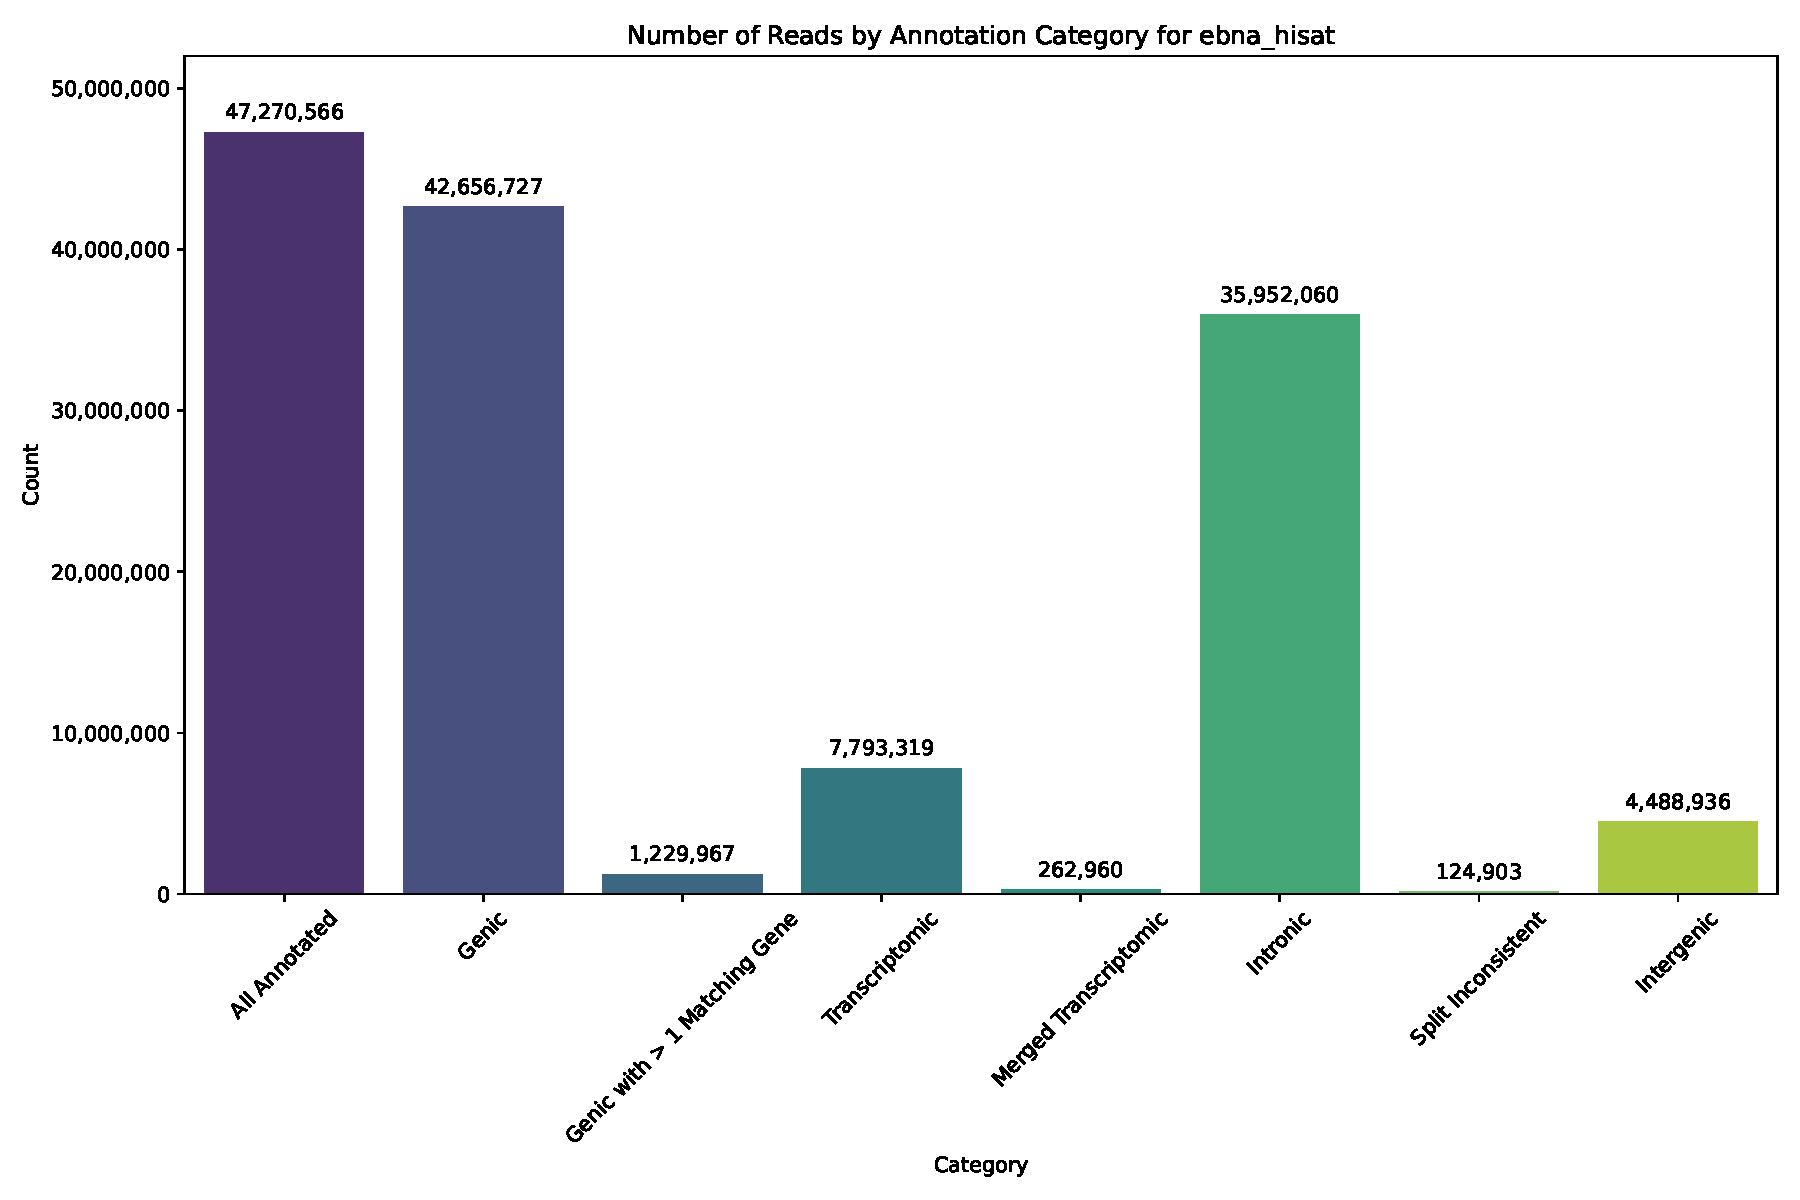
\includegraphics[width=\textwidth]{figures/BamFeatures/annot/ebna_hisat_annotation_counts}
            \label{fig:ebna_hisat_annotation_counts}
        \end{minipage}
        \hfill
        \begin{minipage}{0.32\textwidth}
            \centering
            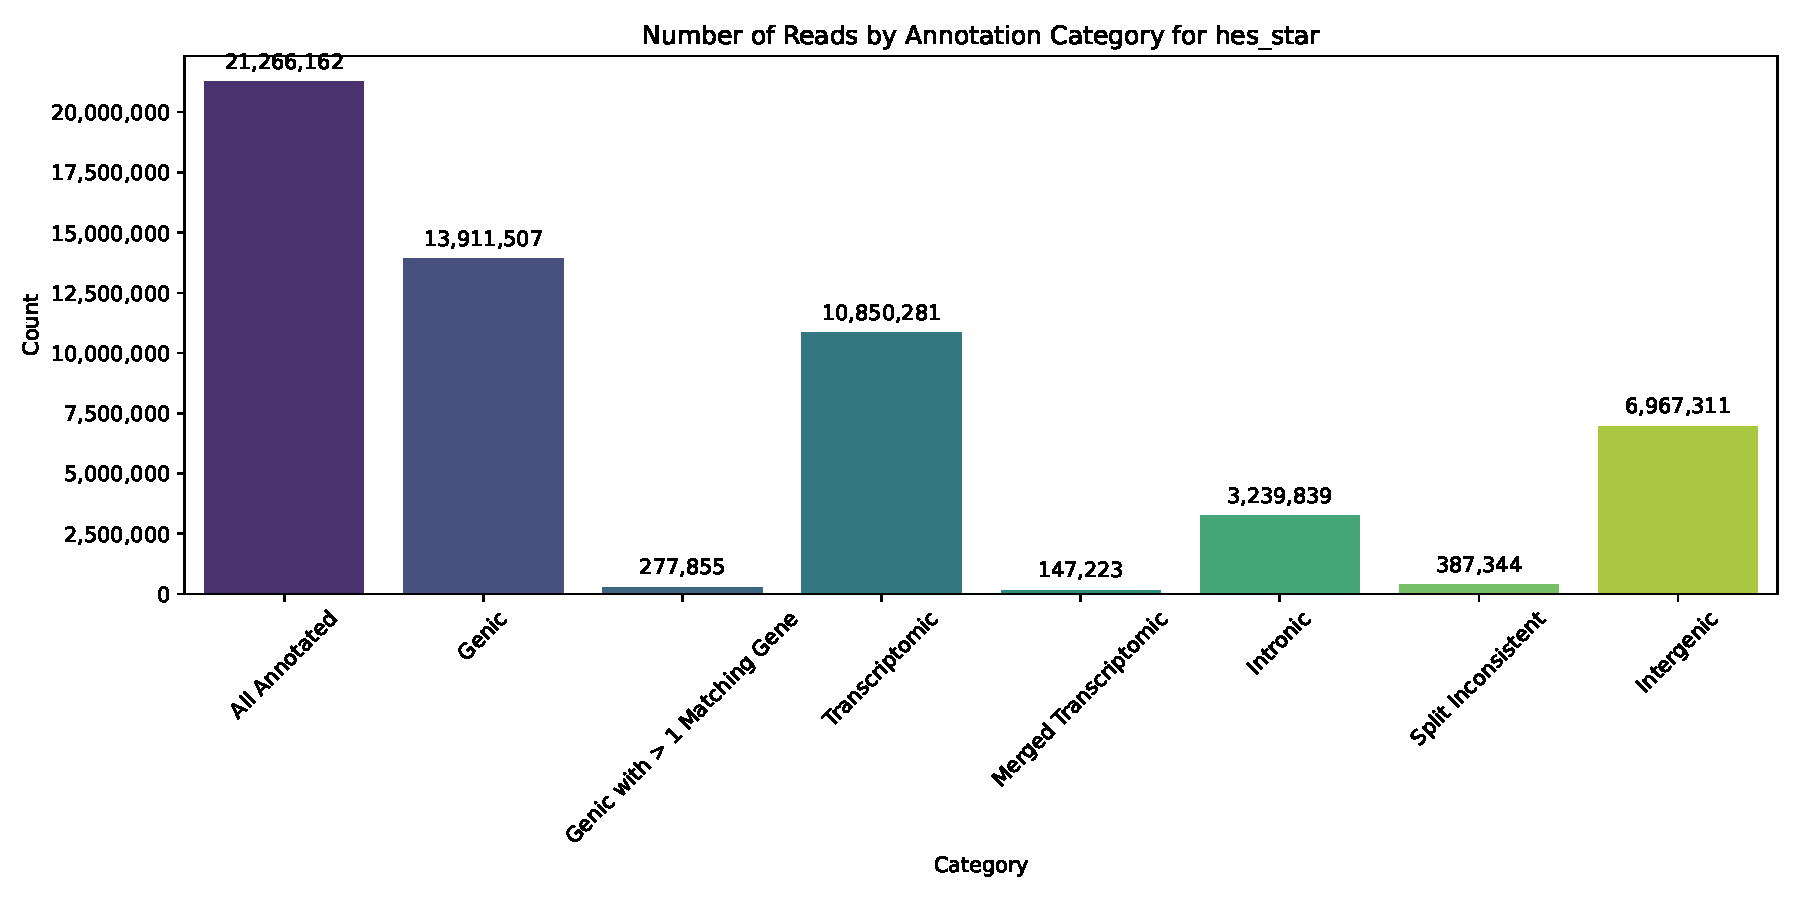
\includegraphics[width=\textwidth]{figures/BamFeatures/annot/hes_star_annotation_counts}
            \label{fig:hes_star_annotation_counts}
        \end{minipage}
        \hfill
        \begin{minipage}{0.32\textwidth}
            \centering
            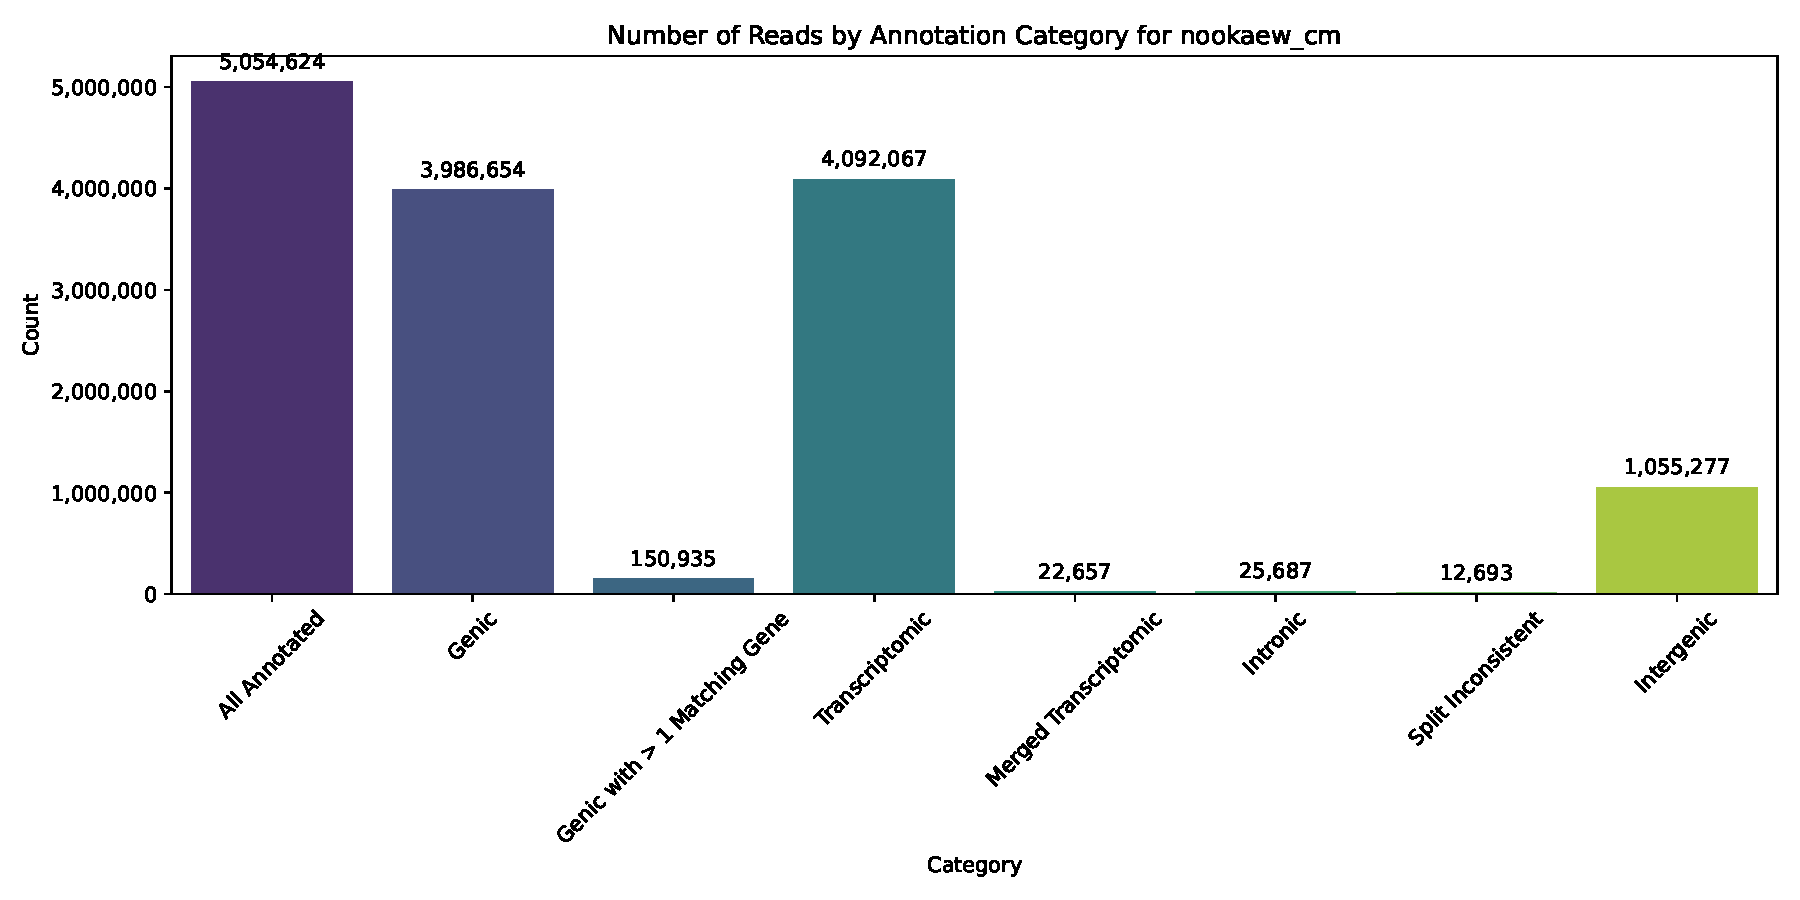
\includegraphics[width=\textwidth]{figures/BamFeatures/annot/nookaew_cm_annotation_counts}
            \label{fig:nookaew_cm_annotation_counts}
        \end{minipage}
        \caption{Comparison of read counts across annotation categories for the provided analysis files. Categories include genic regions, intergenic regions, transcripts, introns, and inconsistent annotations, with the total annotated reads being the sum of genic, intergenic, and split inconsistent categories. The \textit{ebna\_hisat} dataset exhibits a high proportion of intronic reads, indicating significant transcriptional activity in non-coding regions. Similarly, \textit{hes\_star} shows a substantial intronic component, though to a lesser extent. In contrast, the \textit{nookaew\_cm} dataset, derived from yeast, contains very few intronic reads, reflecting the compact genome organization of yeast with minimal intronic sequences.}
        \label{fig:annotation-counts}
    \end{figure}
% TODO: Better caption

    \subsubsection{PCR Index Distribution}
    The cumulative distributions of PCR index counts for three datasets were analyzed, as shown in Figure~\ref{fig:pcr-index}. The \textit{ebna\_hisat} experiment spans PCR index counts up to approximately 3,000,000, while \textit{hes\_star} reaches over 1,000,000, driven largely by a single outlier read with a PCR index of 1,063,959. In contrast, the \textit{nookaew\_cm} dataset has a much smaller range, with PCR index values capped below 200. These differences highlight substantial variability in amplification dynamics across datasets.

    %pcr index distribution
    \begin{figure}[!htbp]
        \centering
        \begin{minipage}{0.32\textwidth}
            \centering
            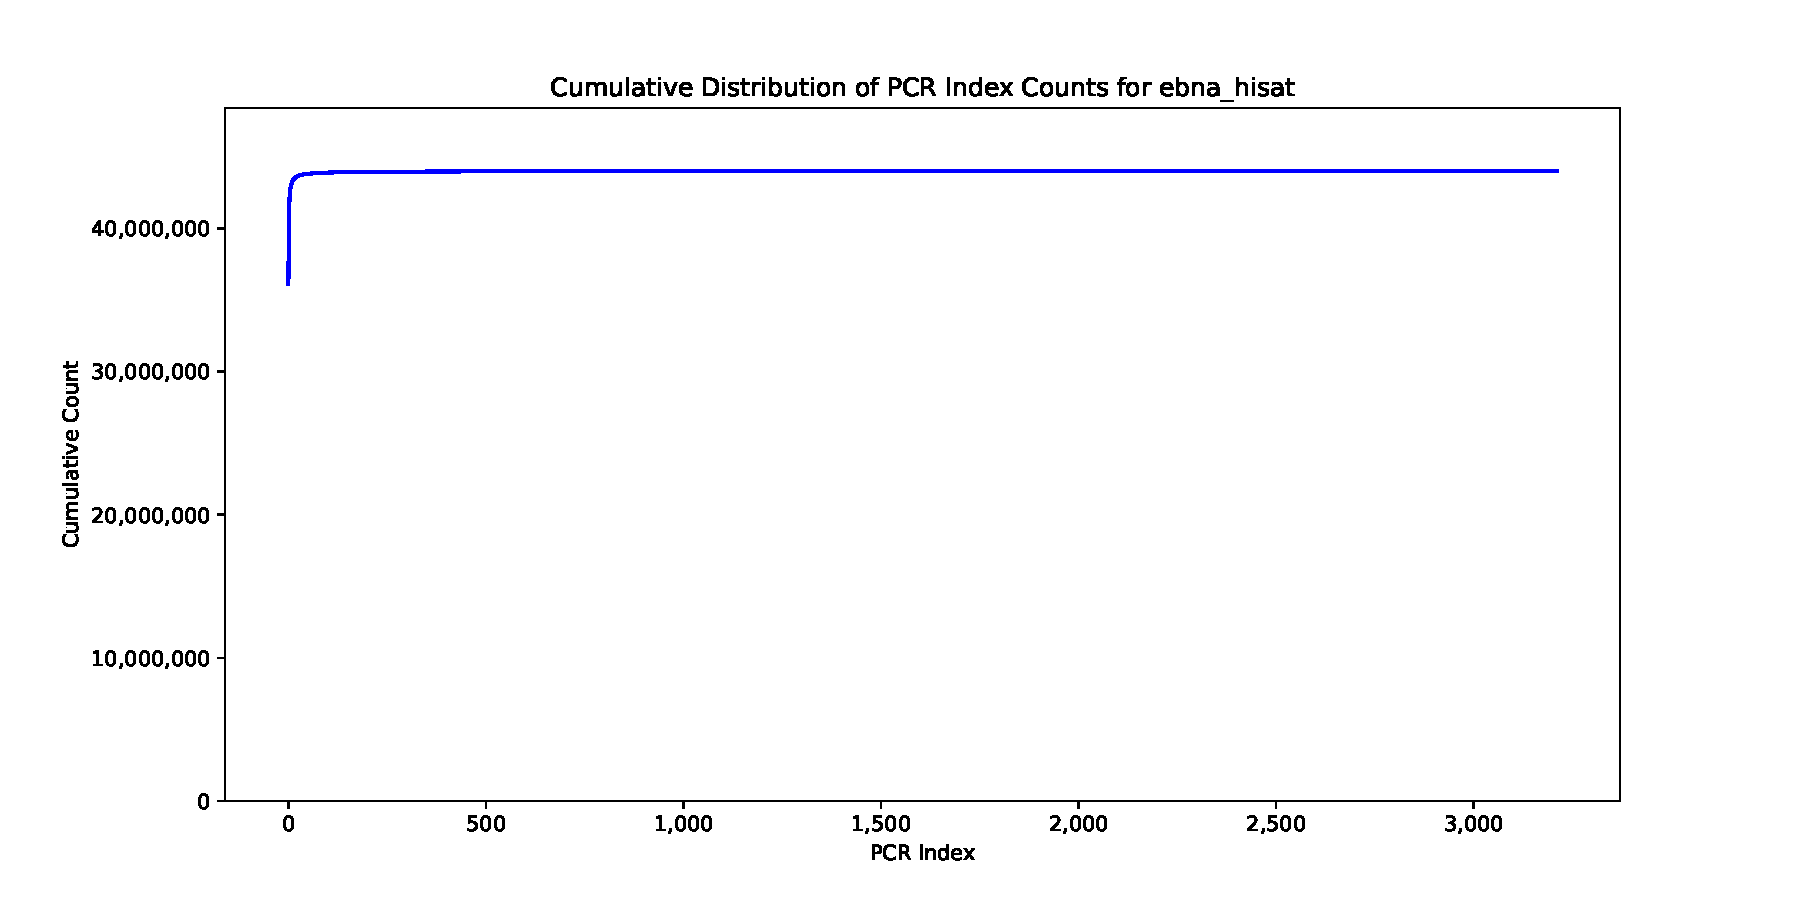
\includegraphics[width=\textwidth]{figures/BamFeatures/annot/ebna_hisat_pcr_index_distribution}
            \label{fig:ebna_hisat_pcr_index_negative_binomial_fit}
        \end{minipage}
        \hfill
        \begin{minipage}{0.32\textwidth}
            \centering
            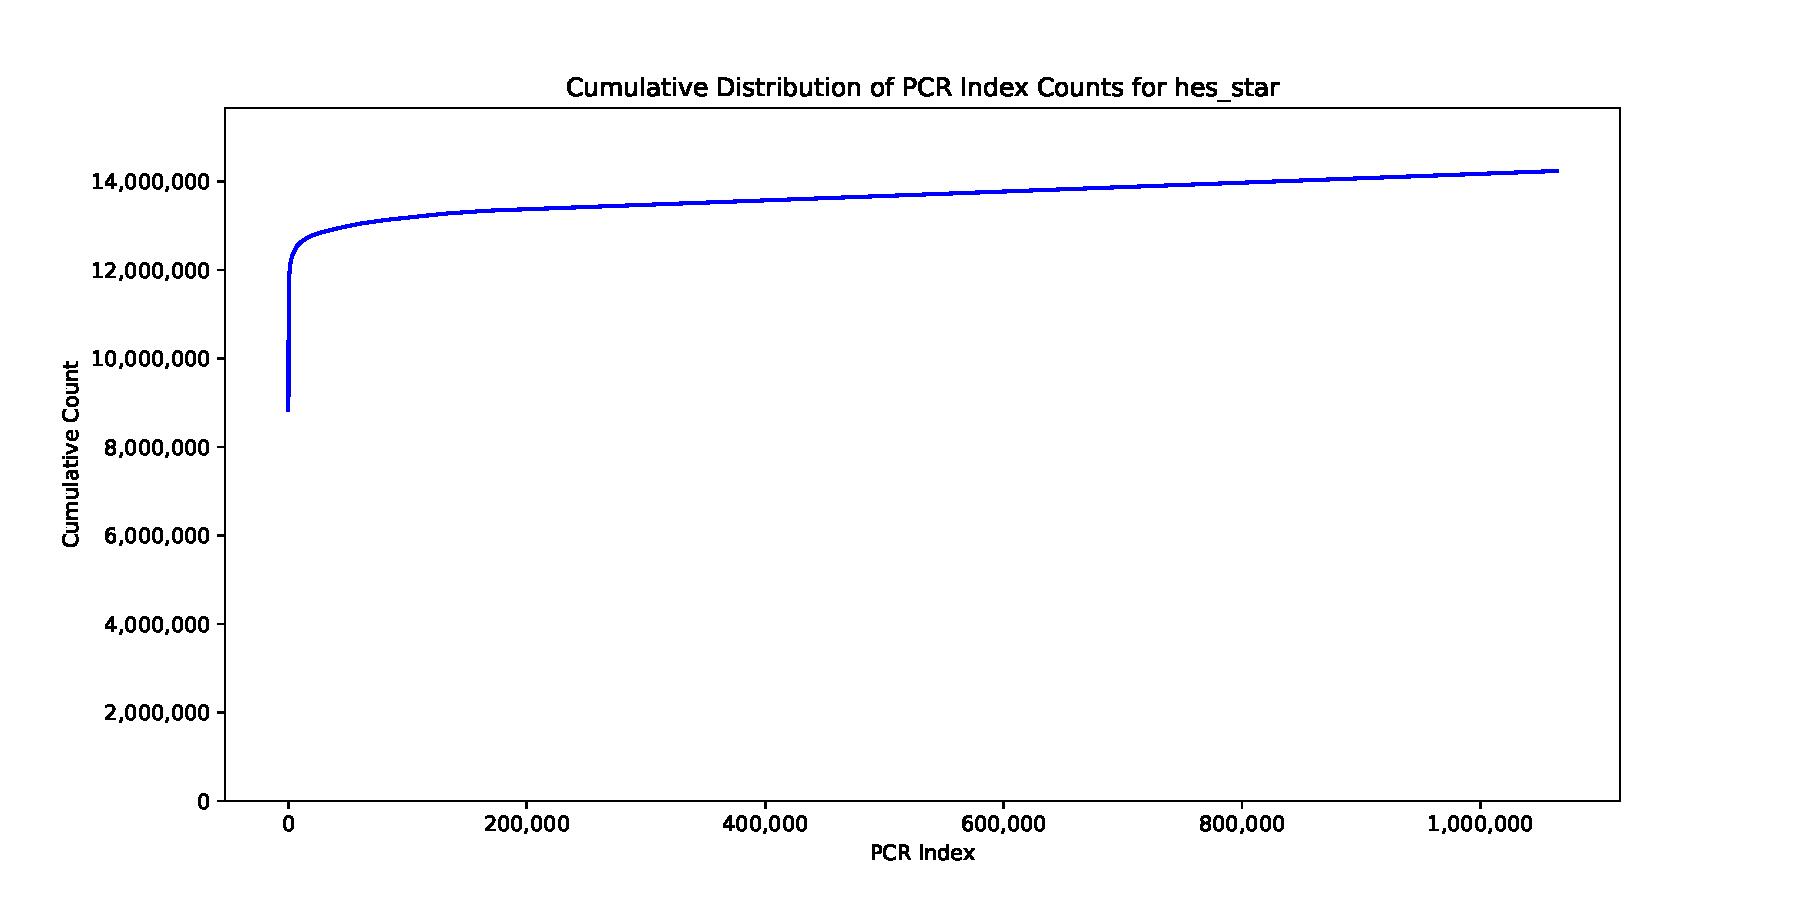
\includegraphics[width=\textwidth]{figures/BamFeatures/annot/hes_star_pcr_index_distribution}
            \label{fig:hes_star_pcr_index_negative_binomial_fit}
        \end{minipage}
        \hfill
        \begin{minipage}{0.32\textwidth}
            \centering
            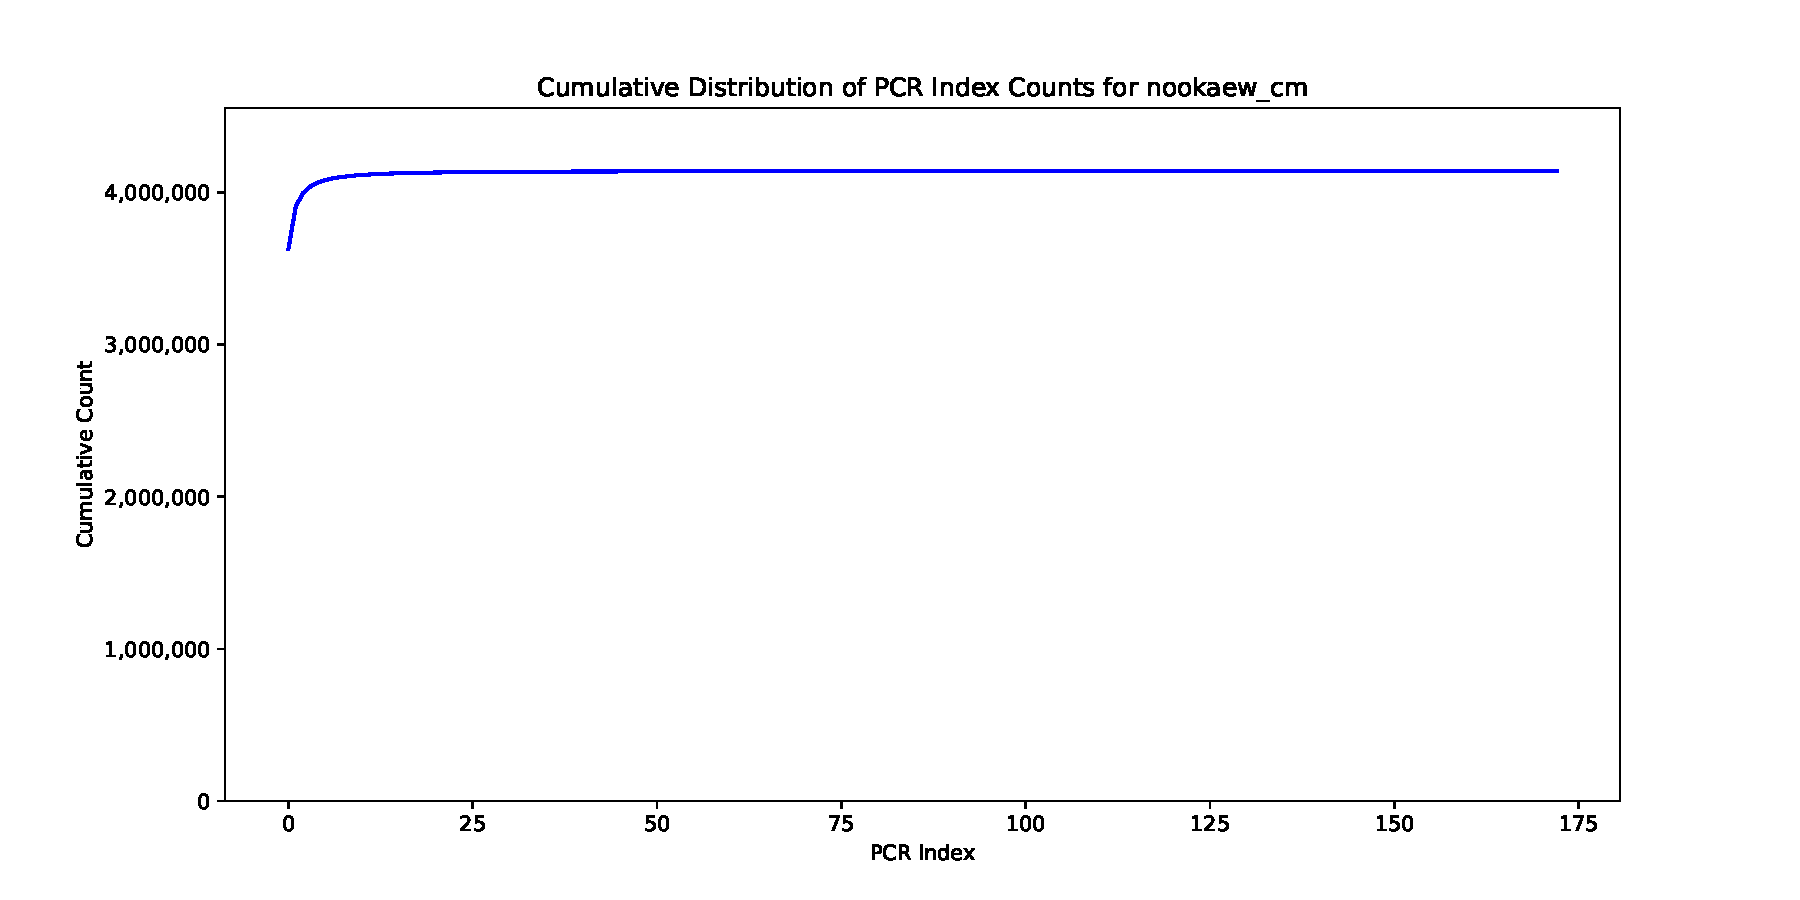
\includegraphics[width=\textwidth]{figures/BamFeatures/annot/nookaew_cm_pcr_index_distribution}
            \label{fig:nookaew_cm_pcr_index_negative_binomial_fit}
        \end{minipage}
        \caption{Cumulative distributions of PCR index counts for the provided analysis files. The x-axis represents the PCR index values, and the y-axis shows the cumulative count of reads. The blue line shows the empirical cumulative distribution. Notably, the x-axis scale differs significantly across datasets: \textit{ebna\_hisat} and \textit{hes\_star} span thousands or hundreds of thousands of PCR index counts, whereas \textit{nookaew\_cm} spans fewer than 200. However, the x-axis is extremely distorted in the \textit{hes\_star} experiment by single read with a max PCR index of 1,063,959 }

        \label{fig:pcr-index}
    \end{figure}
    To model the PCR Index distributions, various distributions were tested, including the Poisson, negative binomial, and gamma distributions. However, no distribution provided a perfect fit for the data without explicitly modeling the parameters of the distribution after the results annotation. Modeling using the negative binomial distribution fitted better than the other distributions tested, with the parameters $r$ and $p$ calculated through the known variance and mean of the experiment.

    \subsubsection{Gene Distance Distribution}
    The cumulative distribution functions (CDFs) of distances from reads to the nearest annotated gene are shown in Figure~\ref{fig:gdist-cdf}. The x-axis represents the distance to the nearest gene in base pairs, while the y-axis shows the cumulative probability. For all datasets, the majority of intergenic reads are located very close to annotated genes, as indicated by the steep initial rise in the CDFs. This pattern suggests potential annotation issues, such as unannotated intronic retention events or the presence of novel transcripts.
    % gdist distribution
    \begin{figure}[!htbp]
        \centering
        \begin{minipage}{0.32\textwidth}
            \centering
            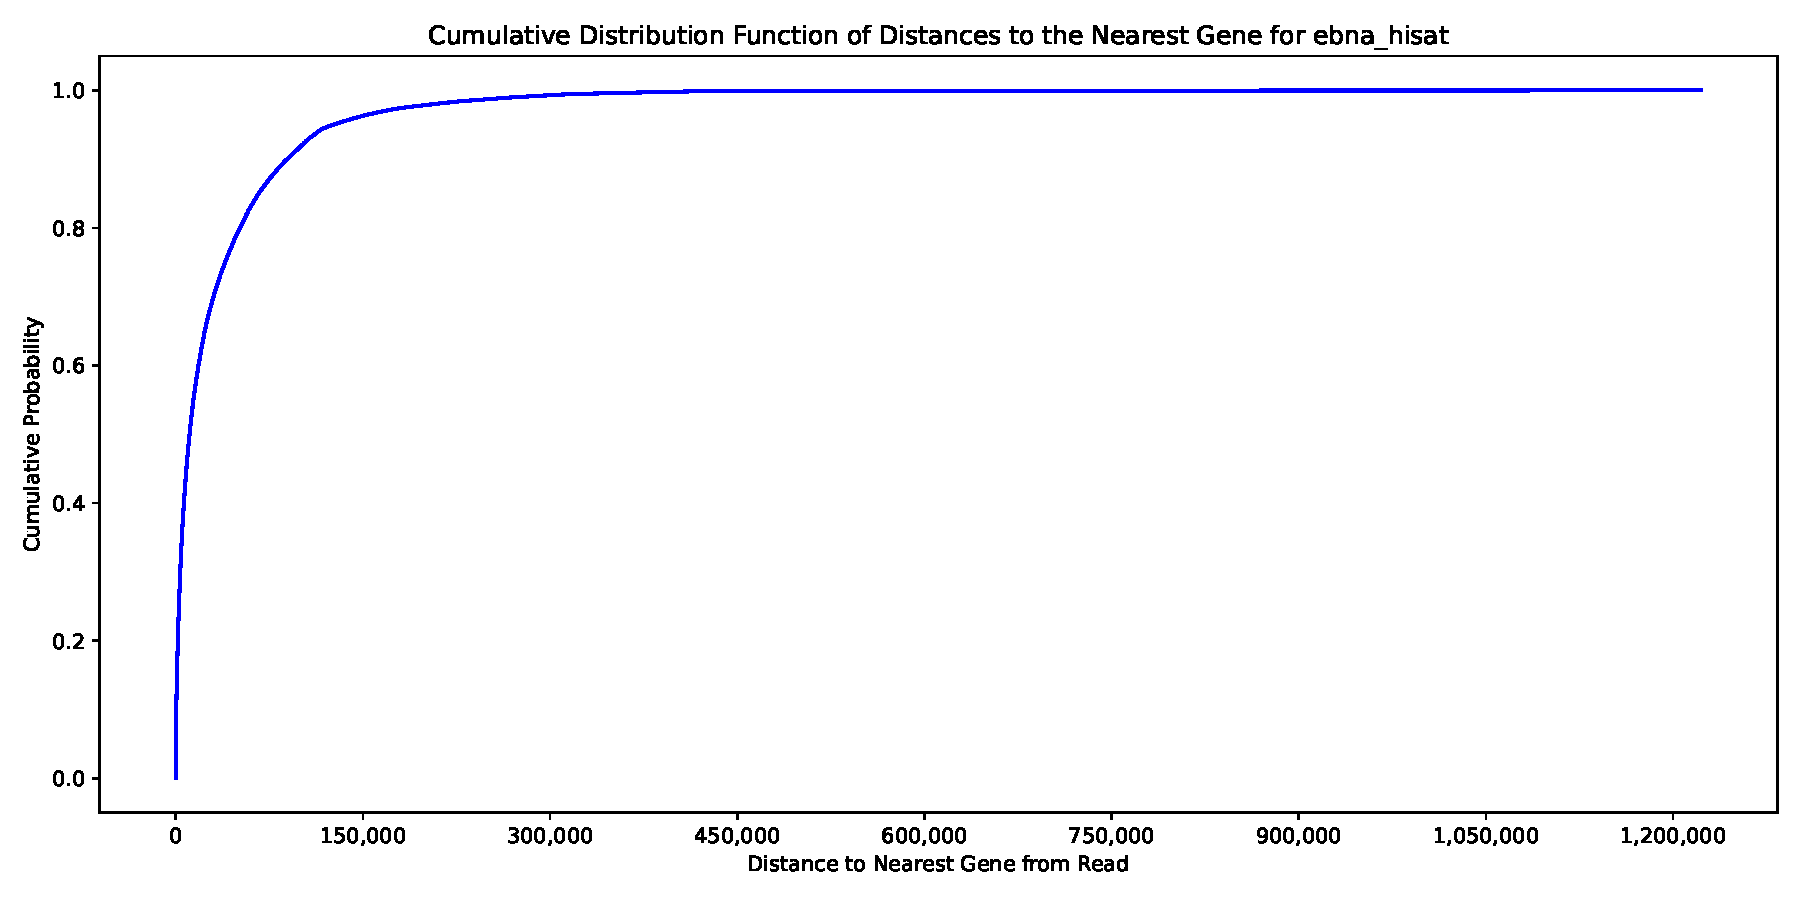
\includegraphics[width=\textwidth]{figures/BamFeatures/annot/ebna_hisat_gdist_cdf}
            \label{fig:ebna_hisat_gdist_cdf}
        \end{minipage}
        \hfill
        \begin{minipage}{0.32\textwidth}
            \centering
            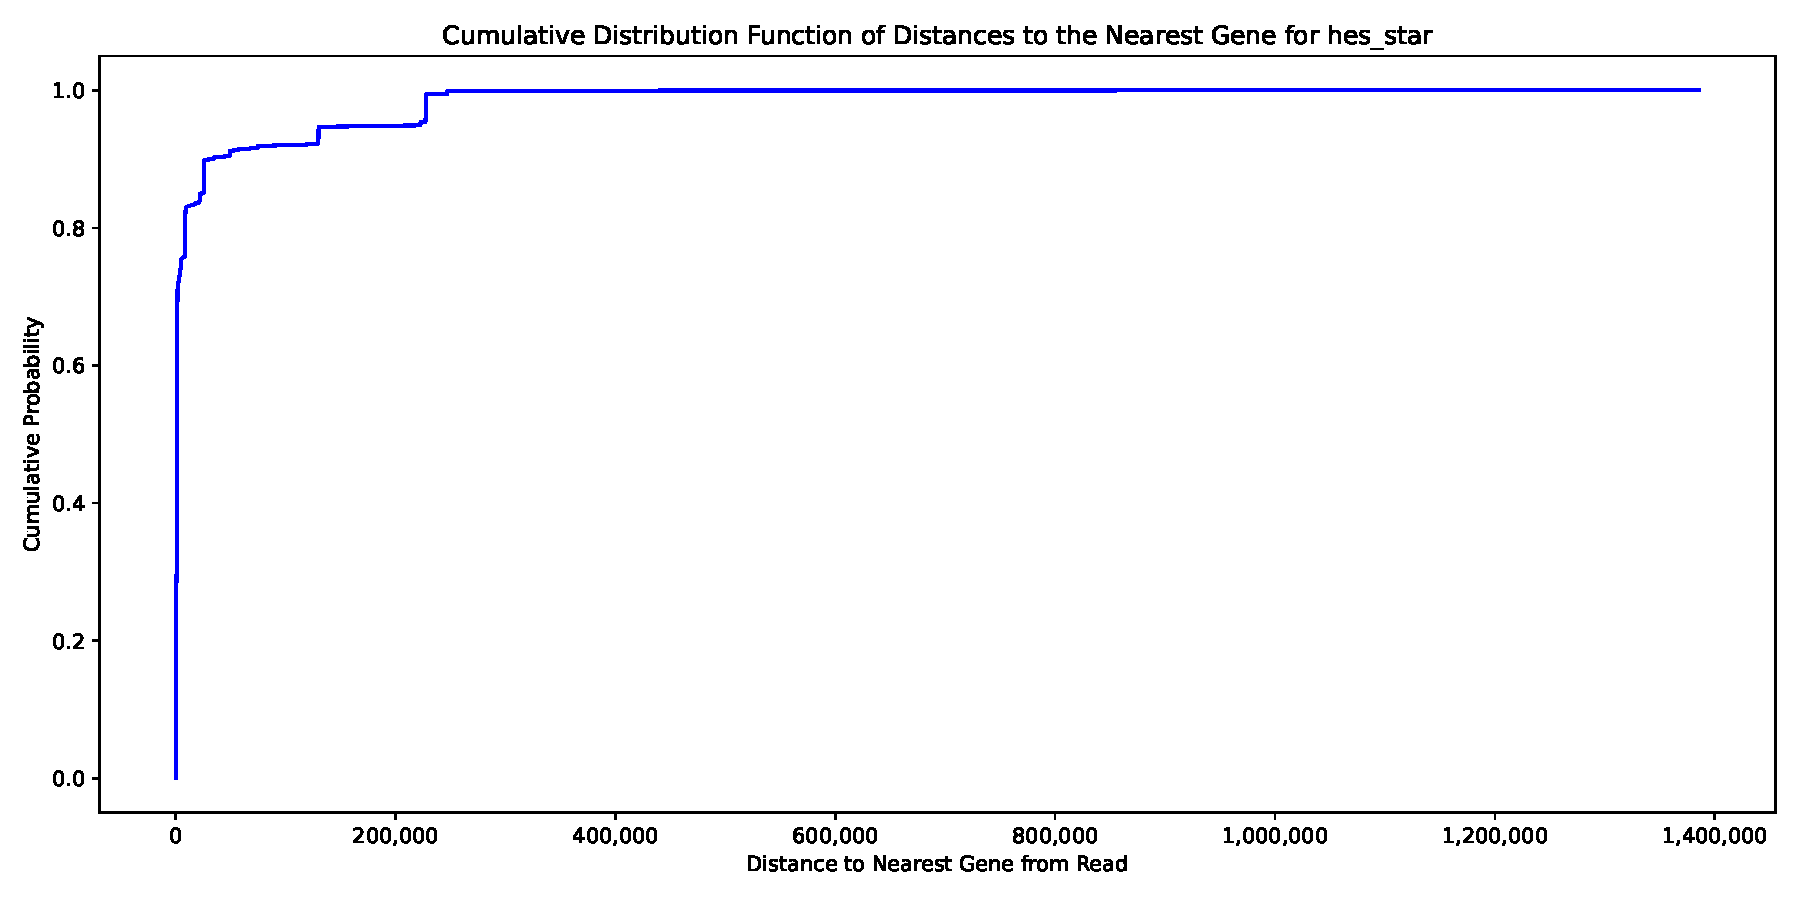
\includegraphics[width=\textwidth]{figures/BamFeatures/annot/hes_star_gdist_cdf}
            \label{fig:hes_star_gdist_cdf}
        \end{minipage}
        \hfill
        \begin{minipage}{0.32\textwidth}
            \centering
            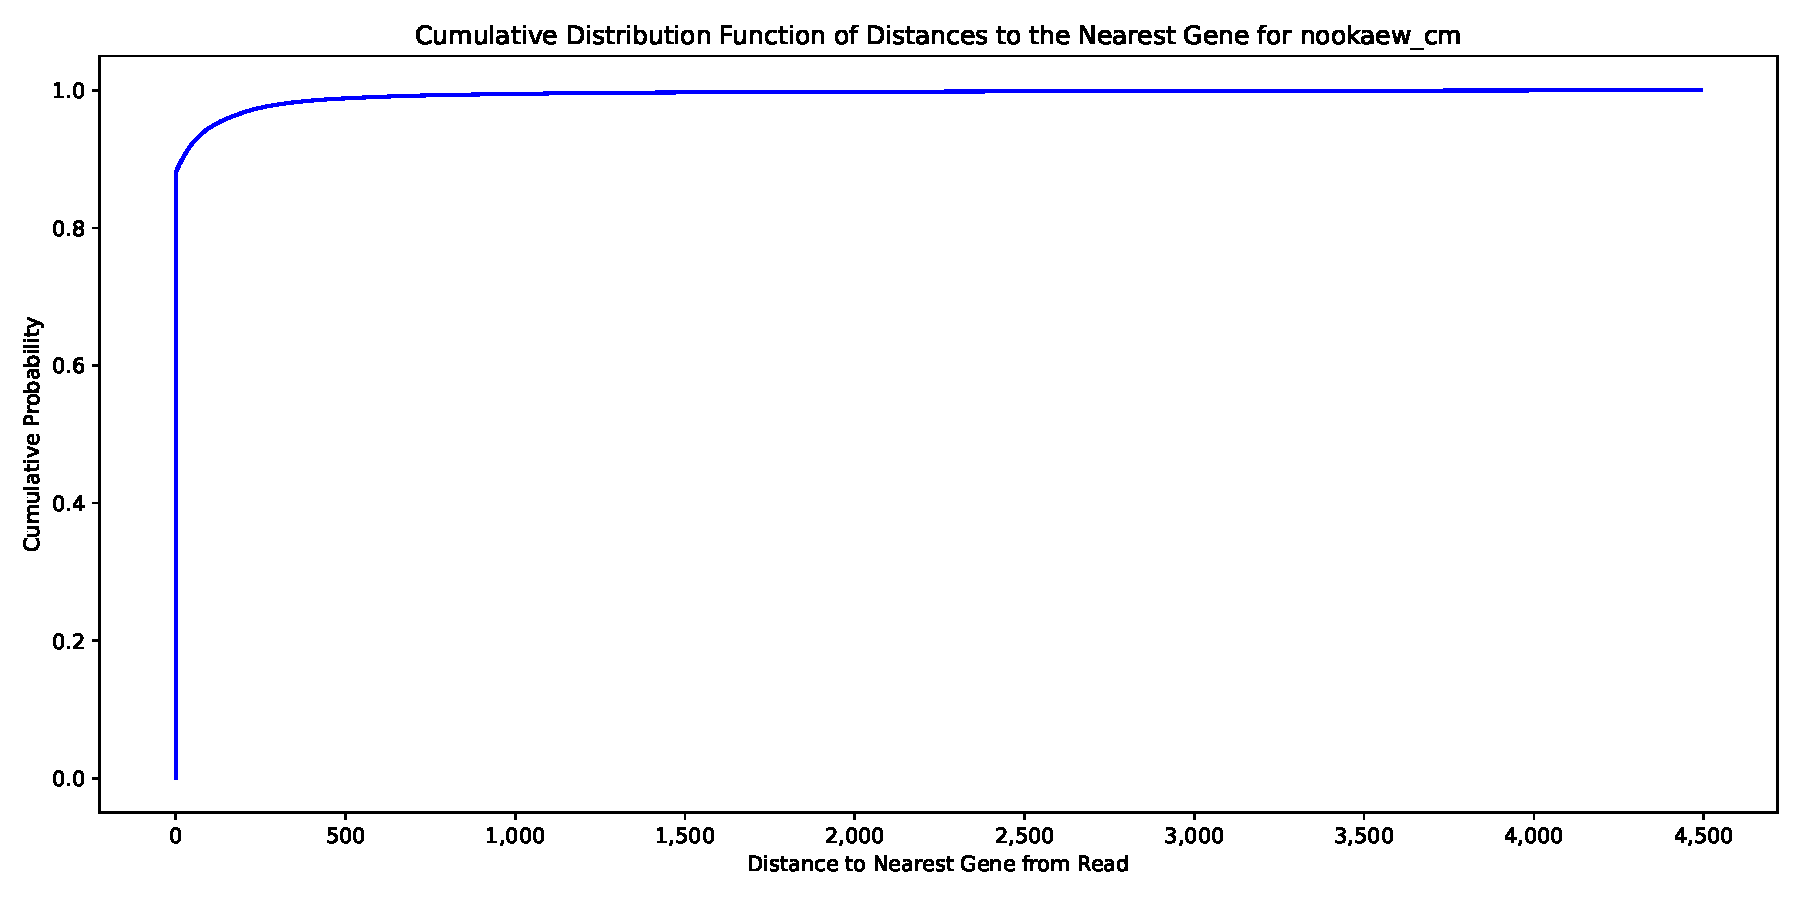
\includegraphics[width=\textwidth]{figures/BamFeatures/annot/nookaew_cm_gdist_cdf}
            \label{fig:nookaew_cm_gdist_cdf}
        \end{minipage}
        \caption{Cumulative distribution functions (CDFs) of distances from reads to the nearest annotated gene for the provided analysis files.. The x-axis represents the distance to the nearest gene in base pairs, while the y-axis shows the cumulative probability. For all datasets, the majority of intergenic reads are located very close to annotated genes, as indicated by the steep initial rise in the CDFs. This suggests the possibility of annotation errors, such as unannotated intronic retention events or novel transcripts. Notably, the scale of the x-axis varies, with \textit{nookaew\_cm} (yeast) showing much smaller distances compared to the human datasets (\textit{ebna\_hisat} and \textit{hes\_star}), consistent with the compact nature of the yeast genome.}
        \label{fig:gdist-cdf}
    \end{figure}
    The x-axis scale varies significantly across datasets, reflecting differences in genome organization. In the \textit{nookaew\_cm} dataset (yeast), distances to the nearest gene are generally much smaller, consistent with the compact nature of the yeast genome. In contrast, the \textit{ebna\_hisat} and \textit{hes\_star} datasets (human) exhibit larger distances, as expected given the greater prevalence of intergenic regions in the human genome. Despite these differences, the sharp rise in the CDFs near zero for all datasets highlights that most reads align close to genes. This observation supports the notion that many intergenic reads may originate from unannotated genomic features, which could include novel transcripts or retained introns.
    The large number of annotated reads that have a distance of zero, is largely due to reads that are partially overlapping with the gene. This is due to the way the program calculates the distance, by finding the closest gene to the read pair. If the read pair is partially overlapping with the gene, the distance is zero. This suggests the reliance of gene rich regions for the mapper. The gradual tailing of the distributions in the human experiments displays a subset of reads that are likely 'truly' from intergenic regions, possibly from ncRNAs or other unannotated regions.

    \subsubsection{JUnit tests}
    When optimizing the program for performance, this testing suite helps verify that improvements do not compromise
    correctness. By running this test after performance-related modifications, we ensure that our changes do not affect
    the accuracy.
    A JUnit test was implemented in order to test the correctness of the program by comparing it to the reference
    solutions. In order to run the tests for all provided BAM files with annotations, a reference table format is used (Table \ref{tab:ref-table-format}). The reference solution is read, storing the lines in a map by read ID. When we process a new line in our program's solution, we compare it to the reference solution and remove it from the map. If the annotation does not match, an error is thrown, and the test fails. The testing suite is robust and ignores trivial differences, such as a different order of the listed genes in the transcriptomic case. If we don't find the read ID of the currently processed line of our solution, an error is thrown. Additionally, once we finish processing our solution, if there are still entries in the reference solution map, it means that we are missing a read ID, and the test also fails.

    \begin{table}[]
        \centering
        \captionsetup{skip=10pt} % Adjust the space between caption and table (default is 10pt)
        \caption
        {Reference Table Format. Columns are separated by tabs. Bam: the name of the BAM file. gtf: The corresponding
        annotation file in GTF format. strandness: Specifies the strandness of the experiment. If the strandness is not
        given, this column will be empty. reference\_solution: The reference solution associated with the experiment.}
        \label{tab:ref-table-format}
        \resizebox{0.7\textwidth}{!}{%
            \begin{tabular}{|l|l|l|l|}
                \hline
                \textbf{bam} & \textbf{gtf} & \textbf{strandness} & \textbf{reference\_solution} \\ \hline
            \end{tabular}%
        }
    \end{table}

    \subsubsection{Feature Counts}
    In order to properly compare the results of the program, the \texttt{featureCounts} method in R was used \cite{liao_smyth_shi_2013}. The tool calculates the count of each feature (gene) per Read Pair. The parameters used for the program are listed in the Supplement \ref{sec:feature-counts-usage}. The results were then converted to RPKM values using the formula in Figure \ref{eq:rpkm}. The top 10 genes for each program were then compared. The results are shown in Table \ref{tab:feature-counts-comparison}. The top 10 genes for each program are similar, with some overlap. However, it is important to note that it is not possible to configure \texttt{featureCounts} to perform in the same way as our program. For example, merged transcriptomic and intronic read pairs are not assigned to a gene. For example, \texttt{ebna\_hist} has a very large proportion of intronic matches, which naturally won't be found by the \texttt{featureCounts} method. This can be used as a sanity check but cannot be used to certify the program's correctness. Naturally, there are many ambiguities when solving this problem where it is not clear what should be done with a certain read or what exactly to count into the RPKM value. Likewise, if this assignment were to be solved by 100 talented programmers, you would likely get 100 different but similar answers.
    \begin{table}[]
        \centering
        \caption{Top 10 Total RPKM values obtained from the program described in this paper are obtained from the feature counts of the featureCounts package in R, converted to RPKM. Gene Names in bold mean that the gene is present in the top 10 of the other program, respectively. The left column is the program described in this paper, and the right column is the featureCounts results. There is a significant overlap between the top 10 values.}
        \label{tab:feature-counts-comparison}
        \resizebox{\textwidth}{!}{%
            \begin{tabular}{cc|cc|cc}
                \multicolumn{2}{c|}{\textbf{ebna\_hist}} &
                \multicolumn{2}{c|}{\textbf{hes\_star}} &
                \multicolumn{2}{c}{\textbf{nookaew\_cm}} \\ \hline
                \multicolumn{1}{c|}{BAMFeatures} &
                featureCounts &
                \multicolumn{1}{c|}{BAMFeatures} &
                featureCounts &
                \multicolumn{1}{c|}{BAMFeatures} &
                featureCounts \\ \hline
                \multicolumn{1}{c|}{ENSG00000234883} &
                \textit{\textbf{ENSG00000202198}} &
                \multicolumn{1}{c|}{\textit{\textbf{ENSG00000251705}}} &
                \textit{\textbf{ENSG00000251705}} &
                \multicolumn{1}{c|}{YGR192C} &
                \textit{\textbf{YLR167W}} \\ \hline
                \multicolumn{1}{c|}{\textit{\textbf{ENSG00000202198}}} &
                \textit{\textbf{ENSG00000238622}} &
                \multicolumn{1}{c|}{\textit{\textbf{ENSG00000210082}}} &
                ENSG00000239776 &
                \multicolumn{1}{c|}{\textit{\textbf{YKL060C}}} &
                \textit{\textbf{YKL060C}} \\ \hline
                \multicolumn{1}{c|}{ENSG00000226779} &
                ENSG00000269900 &
                \multicolumn{1}{c|}{\textit{\textbf{ENSG00000211459}}} &
                ENSG00000241781 &
                \multicolumn{1}{c|}{YBR118W} &
                YDR524C-B \\ \hline
                \multicolumn{1}{c|}{ENSG00000249335} &
                ENSG00000251562 &
                \multicolumn{1}{c|}{ENSG00000206596} &
                ENSG00000200434 &
                \multicolumn{1}{c|}{YHR174W} &
                \textit{\textbf{YLR110C}} \\ \hline
                \multicolumn{1}{c|}{ENSG00000233844} &
                ENSG00000265695 &
                \multicolumn{1}{c|}{ENSG00000206652} &
                \textbf{ENSG00000210082} &
                \multicolumn{1}{c|}{\textit{\textbf{YKL152C}}} &
                YDR524W-C \\ \hline
                \multicolumn{1}{c|}{ENSG00000026508} &
                ENSG00000266019 &
                \multicolumn{1}{c|}{ENSG00000163046} &
                ENSG00000209082 &
                \multicolumn{1}{c|}{\textit{\textbf{YLR167W}}} &
                YKL153W \\ \hline
                \multicolumn{1}{c|}{\textit{\textbf{ENSG00000238622}}} &
                ENSG00000265150 &
                \multicolumn{1}{c|}{\textit{\textbf{ENSG00000202198}}} &
                \textit{\textbf{ENSG00000211459}} &
                \multicolumn{1}{c|}{YLR044C} &
                YLR076C \\ \hline
                \multicolumn{1}{c|}{ENSG00000258486} &
                ENSG00000263900 &
                \multicolumn{1}{c|}{\textit{\textbf{ENSG00000258486}}} &
                ENSG00000265150 &
                \multicolumn{1}{c|}{YLR075W} &
                YDL133C-A \\ \hline
                \multicolumn{1}{c|}{ENSG00000256725} &
                ENSG00000211593 &
                \multicolumn{1}{c|}{ENSG00000226958} &
                \textit{\textbf{ENSG00000258486}} &
                \multicolumn{1}{c|}{YOL086C} &
                \textit{\textbf{YKL152C}} \\ \hline
                \multicolumn{1}{c|}{ENSG00000164330} &
                ENSG00000211595 &
                \multicolumn{1}{c|}{ENSG00000198804} &
                \textit{\textbf{ENSG00000202198}} &
                \multicolumn{1}{c|}{\textit{\textbf{YLR110C}}} &
                YHL015W
            \end{tabular}%
        }
    \end{table}

    \subsection{Time}
    The runtime of the program depends on 1) the number of records in the BAM File and 2) the size of the GTF file. However, for large BAM files, the processing of the GTF File can be disregarded since the GTF File is a constant size and much quicker to parse than the BAM File. The runtime of the program was measured for the provided BAM files and is shown in Table \ref{tab:test-bam-runtime}. The runtime of the program was also measured for the BAM files with reference solutions and is shown in Table \ref{tab:reference-bam-runtime}. Compared to \texttt{hes\_star}, processing \texttt{ebna\_hist} takes ~2.5 times longer, while only having ~2.2 more annotations. However, multiple reasons can lead to this discrepancy. Firstly, \texttt{ebna\_hist} has a far larger proportion of intronic reads, which require far more processing than transcriptomic reads as the merged transcriptome needs to be created. Additionally, \texttt{hes\_star} has far more split inconsistent reads, even though it is a smaller file. Split inconsistent reads are comparatively quick to process, as they are only checked for consistency and then outputted. Due to this, it is reasonable to conclude that the runtime of the program is linear in the amount of records. The runtime of \texttt{nookaew\_cm} is much shorter than the human experiments.



    \begin{table}[]
        \centering
        \caption{List of the BAM files provided with the respective gtf, experiment strandness, and the runtime (excluding GTF Parsing). The BAM file were processed on the bioclient grid (write/read to/from HDD) with -Xmx10g and queued with QueueGridForRefTable.sh}
        \label{tab:test-bam-runtime}
        \resizebox{\textwidth}{!}{%
            \begin{tabular}{l|l|l|l|l}
                \textbf{BAM} & \textbf{GTF}                         & \textbf{Strandness} & \textbf{Runtime (seconds)} & \textbf{Number of Annotated Reads} \\ \hline
                ebna\_hisat  & Homo\_sapiens.GRCh37.75              & true                & 325.619                    & 47,270,566                         \\ \hline
                hes\_star    & Homo\_sapiens.GRCh37.75              & false               & 129.077                    & 21,266,162                         \\ \hline
                nookaew\_cm  & Saccharomyces\_cerevisiae.R64-1-1.75 & null                & 29.621                     & 5,054,624
            \end{tabular}%
        }
    \end{table}


    \begin{table}[]
        \centering
        \caption{List of the BAM files provided that have reference solutions with the respective gtf, experiment strandness, and the runtime (excluding GTF Parsing). The BAM files were processed on the bioclient grid (write/read to/from HDD) with -Xmx10g and queued with QueueGridForRefTable.sh}
        \label{tab:reference-bam-runtime}
        \resizebox{\textwidth}{!}{%
            \begin{tabular}{l|l|l|l|l}
                \textbf{BAM} & \textbf{GTF}                         & \textbf{Strandness} & \textbf{Runtime (seconds)} & \textbf{Number of Annotated Reads} \\ \hline
                y.ns.2       & Saccharomyces\_cerevisiae.R64-1-1.75 & null                & 0.350                      & 20,876                             \\ \hline
                y.ns.5       & Saccharomyces\_cerevisiae.R64-1-1.75 & null                & 0.372                      & 18,505                             \\ \hline
                h.sn.1       & Homo\_sapiens.GRCh37.75              & false               & 0.336                      & 17,209                             \\ \hline
                h.sn.7       & Homo\_sapiens.GRCh37.75              & false               & 0.340                      & 16,116                             \\ \hline
                h.sp.3       & Homo\_sapiens.GRCh37.75              & true                & 0.375                      & 22,806                             \\ \hline
                h.sp.8       & Homo\_sapiens.GRCh37.75              & true                & 0.425                      & 21,092
            \end{tabular}%
        }
    \end{table}


    \section{Supplement}

    \subsection{Feature Counts Usage}\label{sec:feature-counts-usage}
    \begin{verbatim}

counts <- featureCounts(
  files = bam_file,
  annot.ext = annotation_file,
  isGTFAnnotationFile = TRUE,
  GTF.featureType = "exon",
  GTF.attrType = "gene_id",
  useMetaFeatures = TRUE,
  isPairedEnd = TRUE,
  countMultiMappingReads = FALSE,
  nthreads = 8,
  allowMultiOverlap = TRUE,
  primaryOnly = TRUE,
  strandSpecific = -, # Depends on the experiment 0=null, 1=true, 2=false
  requireBothEndsMapped = TRUE,
  countReadPairs = TRUE,
  countChimericFragments = FALSE,
)
    \end{verbatim}

    \AtNextBibliography{\small}
    \printbibliography
\end{document}
